\documentclass[a4paper,11pt,twoside]{report}

\usepackage[utf8]{inputenc} 
\usepackage[T1]{fontenc}      
\usepackage[francais]{babel}
\addto\captionsfrench{\renewcommand{\chaptername}{Partie}}
\usepackage{graphicx}
\usepackage{newcent}
\usepackage{listings}
\usepackage{verbatim}
\usepackage{moreverb}
\usepackage[top=2cm, bottom=2cm, left=2cm, right=2cm]{geometry}

\usepackage{xcolor}
\usepackage{color}
%Définition des couleurs
\definecolor{vert}{HTML}{729928}
\definecolor{vert-fonce}{RGB}{89,120,31}
\definecolor{soft-dark}{RGB}{45,60,16}
\definecolor{vert-clair}{HTML}{99cb38}

\usepackage{etoolbox}
\makeatletter
\patchcmd{\@footnotetext}{\footnotesize}{\scriptsize\sffamily}{}{}
\makeatother
\usepackage{lastpage}
\usepackage{fancyhdr}
\fancypagestyle{plain}{
  \fancyhf{}
  %Définition de l'entête des pages
  \renewcommand{\headrulewidth}{0pt}
  \fancyhead[C]{{\fontfamily{pag}\selectfont\scriptsize\color{vert-fonce}{\textsc{| \leftmark}}}}
  \fancyhead[L]{}
  \fancyhead[R]{}
  %Définition du pied des pages
  \fancyfoot[C]{}
  \fancyfoot[L]{}
  \fancyfoot[R]{\fontfamily{pag}\selectfont\small\color{vert-fonce}{\textsc{| \thepage/\pageref{LastPage}}}}
}
\pagestyle{plain}

\usepackage{titlesec}
%Changement du format des titres des chapitres
\titleformat{\chapter}[hang]{\huge\textcolor{vert}}{\thechapter}{2pc}{}[]
\titleformat{\section}[hang]{\LARGE\textcolor{vert-clair}}{\thesection}{2pc}{}[]
\titleformat{\subsection}[hang]{\Large\textcolor{soft-dark}}{\thesubsection}{2pc}{}[]
\titleformat{\paragraph}[hang]{\sffamily\bfseries}{\theparagraph}{2pc}{}[]

%Changement du format des titres des figures
\usepackage[font={footnotesize,it,sf}]{caption}

%Changement du comportement de la mise en avant d'un élément
\renewcommand{\emph}{\bfseries}

%Changement aspect du label dans les descriptions
\usepackage{enumitem}
\setlist[description]{
  font={\bfseries\sffamily}
}

%Code input
\definecolor{mygreen}{rgb}{0,0.6,0}
\definecolor{mygray}{rgb}{0.5,0.5,0.5}
\definecolor{mymauve}{rgb}{0.58,0,0.82}
\lstset{ %
  backgroundcolor=\color{white},   
  basicstyle=\scriptsize,        % the size of the fonts that are used for the code
  breakatwhitespace=false,         % sets if automatic breaks should only happen at whitespace
  breaklines=true,                 % sets automatic line breaking
  commentstyle=\color{mygreen},    % comment style
  keywordstyle=\color{blue},       % keyword style
  numbers=left,                    % where to put the line-numbers; possible values are (none, left, right)
  numbersep=5pt,                   % how far the line-numbers are from the code
  numberstyle=\tiny\color{mygray}, % the style that is used for the line-numbers
  rulecolor=\color{black},         % if not set, the frame-color may be changed on line-breaks within not-black text (e.g. comments (green here))
  showspaces=false,                % show spaces everywhere adding particular underscores; it overrides 'showstringspaces'
  showstringspaces=false,          % underline spaces within strings only
  showtabs=false,                  % show tabs within strings adding particular underscores
  stepnumber=1,                    % the step between two line-numbers. If it's 1, each line will be numbered
  stringstyle=\color{mymauve},     % string literal style
  tabsize=2,                       % sets default tabsize to 2 spaces
}

\begin{document}
%Font sans empattement 
\sffamily

%Saut de page
\clearpage

\chapter*{Introduction}
\thispagestyle{\chead{}}
\addcontentsline{toc}{chapter}{Introduction}%Ajout de l'élément dans le sommaire
Passionné  par les nouvelles technologies, j'ai recherché un stage dans une entreprise et surtout un secteur qui saurait me combler. Plusieurs types de PFE\footnote{Projet de Fin d'Etude} pouvaient convenir à mes attentes et je souhaitais élargir mes horizons et continuer d'agrandir mon bagage technique. Ayant une attirance plus particulière pour les technologies du Web\footnote{Abréviation pour World Wide Web}, j'ai accepté la proposition de Smile Sud-Ouest en tant que développeur d'applications Web. En effet une SSII\footnote{Société de Services en Ingénierie Informatique, maintenant appelé Entreprise de Services du Numérique (ESN)} offre la possibilité d'acquérir beaucoup de connaissances rapidement et d'engranger de l'expérience à travers des projets divers et variés.\newline

L'ensemble des technologies gravitant autour du Web étant en constantes évolution je savais que ce stage était pour moi l'occasion d'exercer dans un environnement qui me passionne. De plus, dès les entretiens j'ai ressenti la bonne ambiance et la convivialité dans cette agence, ce qui a grandement participé à asseoir ce choix de PFE. La taille conséquente de l'entreprise Smile a aussi contribué à faire ce choix, ayant réalisé mon stage de troisième année dans une PME\footnote{Petite et Moyenne Entreprise} comptant seulement quatre employés, j'avais à coeur de découvrir ce qu'était un grand groupe.\newline 

Ce rapport s’efforcera au mieux de donner à son lecteur une idée précise de mes missions au sein de Smile pour les six mois de stage. Dans une première partie, je présenterai le groupe ainsi que sa position dans le secteur. Je porterai une attention particulière à l'agence Bordeaux où j'ai travaillé ainsi qu'aux diverses missions qui m'ont été proposées. Dans un second temps, j’aborderai les différents projets auxquels j'ai participé, leurs réalisations ainsi que les difficultés rencontrées et leurs solutions. Finalement, la dernière partie fera le bilan de ces six mois de stage et s'ouvrira sur les futurs projets en développement Web de l’entreprise.

\chapter*{Remerciements}
\thispagestyle{\chead{}}
\addcontentsline{toc}{chapter}{Remerciements}%Ajout de l'élément dans le sommaire
Lorem ipsum dolor sit amet, consectetur adipiscing elit. Nullam pharetra sem neque, at lacinia tellus rhoncus sed. Aliquam erat volutpat. Sed in facilisis dolor. Nam gravida purus vel ante auctor, non venenatis mauris scelerisque. Maecenas odio nunc, dapibus eu varius ac, dapibus non diam. Nam a ligula sit amet velit porta auctor. Vestibulum vel luctus eros. Sed vestibulum neque tristique, fringilla felis sed, pharetra dui. Nulla facilisi. Aliquam viverra velit nulla, ut placerat purus auctor vitae. Aenean vitae mauris tristique metus placerat ultrices vel ac magna. Vestibulum massa leo, faucibus nec tincidunt vitae, bibendum vel tortor. Aliquam erat volutpat.

%Table des matières
\tableofcontents
\thispagestyle{\chead{}}

\chapter{Présentation de l'entreprise}
  \section{Contexte}
  Le World Wide Web, littéralement la « toile (d’araignée) mondiale », communément appelé le Web permet de consulter, avec un navigateur, des pages accessibles sur des sites. Des sites il y en avait un seul en août 1991, en 2000 nous en comptions déjà 10 000 000, aujourd'hui c'est plus de 947 000 000. Ce chiffre exorbitant ne cesse d'augmenter de jour en jour et le nombre d'entreprises concevant ces sites augmentent lui aussi inexorablement. Aujourd'hui nous faisons face à de nouvelles problématiques dans le domaine de la création d'applications Web ou sites Web, à savoir une complexité des fonctionnalités demandées, une compatibilité cross-plateformes (PC de bureau, tablette et mobile) mais aussi avec toutes les versions des navigateurs (IE8, IE9, Chrome, Firefox, Safari,...) et des systèmes d'exploitations (Windows, MacOS, Linux, iOS, Android,...) et enfin des performances, en terme de vitesse de chargement des pages, toujours plus rapide.
  
  \section{Groupe Smile}
  Dans ce contexte, Smile est une société d'experts des architectures web et des solutions open source fondée en 1991. Cependant ce n'est qu'à partir de 2001 que Smile commence à construire son expertise des solutions open source\footnote{Désigne un logiciel dans lequel le code source est à la disposition du grand public} : un choix d’avenir que beaucoup de ses concurrents n’osent pas alors entreprendre, mais qui s'avèrera être un choix payant. En France et dans le monde ce sont plus de 700 collaborateurs qui opèrent dans une variété de domaines, Smile étant le premier intégrateur européen de logiciel libre.Dans l'hexagone ce sont 8 agences (Paris, Lyon, Nantes, Bordeaux, Montpellier, Marseille, Lille et Grenoble) qui se partagent les différents projets, auxquels s'ajoutent les 8 autres locaux à l'étranger (Amsterdam, Bruxelles, Genève, Zurich, Casablanca, Kiev, Moscou et Abidjan), pour arriver à un groupe comptant 16 infrastructures à travers le monde.\newline

  Acteur engagé dans les progrès de l’Internet\footnote{Réseau informatique mondial accessible au public comportant des services variés comme le Web notamment} depuis 1995, Smile a réalisé quelques-uns des plus grands sites de l'Internet français, des sites à forte valeur ajoutée et à forte audience. Smile a également été choisie par les plus grandes entreprises françaises pour concevoir, réaliser et maintenir des applicatifs Intranet stratégiques, servant des centaines d'utilisateurs sur des milliers de transactions. On notera par exemple quelques grands clients comme le Ministère de la Culture, la Société Générale, Eiffage Immobilier, Dassault Systèmes, Eurosport, Krys, Carrefour,...\newline
  
  On trouve chez Smile plusieurs corps de métiers :\newline
  \begin{description}

    \item[Ingénierie] Le pôle ingénierie accueille le cœur de métier de l’activité de Smile. Il réunit l’ensemble des équipes en charge de concevoir et de produire les applications web répondant aux besoins des clients.
    \item[Commerce] Le pôle commercial regroupe les trois formes d’activités mises en oeuvre par Smile dans sa recherche de business : la prospection, l’ avant-vente et la fructification.
    \item[Consulting] Le pôle consulting se caractérise par son ouverture et sa polyvalence sur les domaines suivants : Enterprise Content Management (gestion de contenus d’entreprise), Assistance à Maîtrise d’Ouvrage (fonctionnel), Conseil Technique, Business Intelligence (Décisionnel) ,...
    \item[Système] Le pôle système travaille au cœur des Systèmes et Réseaux de Smile et de ses clients. L’équipe œuvre sur la maintenance et l’évolution du système interne de Smile, à tous les niveaux : serveurs, réseaux, messagerie, téléphonie,... Pour l’externe, l’équipe a pour fonction d’assurer l’expertise systèmes et réseaux de Smile (architecture système-réseaux, exploitation, hébergement,...) auprès de ses clients.
    \item[Agence Digitale] L'agence Digitale est une équipe qui travaille pour les clients de Smile à la refonte ou à l’élaboration de leur identité visuelle : e- Marketing, charte graphique, accessibilité, interactivité et animation,... 
    \item[Administratif] Le pôle administratif recouvre des métiers aussi nombreux que variés : comptabilité, contrôle de gestion, finances mais aussi ressources humaines et recrutement ou encore communication et marketing.
    \newline
    
  \end{description}
  
  Pour le pôle ingéniérie qui nous intéresse plus particulièrement on trouve de nombreux métiers là aussi, je me contenterai de les siter sans les détailler un à un :\newline
  \begin{itemize}

    \item Ingénieur études et développement (IED)
    \item Développeur
    \item Chef de projet
    \item Expert technique
    \item Chef de projet fonctionnel
    \item Chef de projet technique
    \item Consultant expert veille IT\footnote{Technologies de l'information et de la communication}
    \item Directeur de projet
    \newline
    
  \end{itemize}
  
  Je reviendrai par la suite sur le rôle de l'IED puisque cela correspond à ma fonctions en tant que stagiaire au sein de Smile.
  
  \section{Agence de Bordeaux}
  A Bordeaux ce sont une quarantaine de collaborateurs, majoritairement ingénieurs, qui développent des applications Web utilisant les CMS\footnote{Content Management System, est un site web disposant de fonctionnalités de publication et offrant en particulier une interface d'administration permettant à un administrateur de site de créer ou organiser du contenu} open source (eZ Publish, Drupal), la solution de e-commerce Magento, mais aussi l’ensemble des solutions Open Source portées par Smile. Récemment le développement de projets Symfony 2\footnote{Framework libre et français écrit en PHP 5 destiné majoritairement aux professionnels du développement permettant de faciliter et d’accélérer la création d'un site web} est venu s'ajouter aux missions de l'agence de Bordeaux notamment dû au fait de l'importance que prend ce framework\footnote{En programmation informatique, un framework ou structure logicielle est un ensemble cohérent de composants logiciels structurels, qui sert à créer les fondations ainsi que les grandes lignes de tout ou d’une partie d'un logiciel} PHP\footnote{Langage de programmation libre principalement utilisé pour produire des pages Web dynamiques. PHP est un langage orienté objet et a permis de créer un grand nombre de sites web célèbres, comme Facebook, YouTube, Wikipedia, Google,... Il est aujourd'hui considéré comme la base de la création des sites Internet dits dynamiques} sur le marché.\newline

  Qui dit développement, dit langage informatique, à Bordeaux il y a majoritairement un langage utilisé à savoir le PHP, même si des projets en Java\footnote{ Langage de programmation informatique orienté objet détenu par la société Oracle}, .Net\footnote{Ensemble de produits et de technologies informatiques de l'entreprise Microsoft pour rendre des applications facilement portables sur Internet} ont déjà et sont encore réalisés. En plus de ceux-ci, sont utilisés au quotidien les langages basiques du Web à savoir HTML5\footnote{HyperText Markup Language 5, langage permettant notamment le développement d'applications Web}, CSS3\footnote{Cascading Style Sheets, langage qui décrit la présentation des documents HTML (couleur, mise en page,...)}, JavaScript\footnote{Langage de programmation de scripts principalement employé dans les pages web interactives} et toutes les variantes ou framework qui y sont liés (jQuery, Sass,...). Quand à l'environnement de travail, toutes les machines des développeurs sont équipés de Linux\footnote{Nom couramment donné à tout système d'exploitation libre fonctionnant avec le noyau Linux} avec une distribution spécifique à Smile. Chacun est libre d'y installer, en plus des logiciels de base fournis, tous les outils nécessaires à son travail de développement. Les locaux sont organisés en open-space afin de faciliter les échanges entre collaborateurs et un regroupement par projet est mis en place toujours dans le même but.
  
  \section{Mes missions au sein de Smile}
  Ma première mission au sein de Smile a été d'installé et de mettre en place mon poste de travail, cela est passé par l'installation du Linux custom sur ma machine ainsi que des logiciels nécessaires au développement. J'ai notamment utilisé PhpStorm comme IDE\footnote{Integrated Development Environment, un environnement de développement est un ensemble d'outils pour augmenter la productivité des programmeurs qui développent des logiciels} ainsi que le navigateur Chrome de Google pour débuguer mes pages WEB. En plus de cela j'ai eu besoin d'outils comme VirtualBox pour simuler des environnements Windows à des fins de test de compatibilité, ou encore Meld un logiciel de comparaison de fichier très utile pour détecter des erreurs dans le code. S'en est suivi une période d'autoformation sur les différentes technologies utilisées par l'agence, à savoir Drupal, Magento et EzPublish.\newline 
    
  J'ai par la suite été placé sous la tutelle d'un chef de projet avec qui j'ai commencé le développement pour des clients sur des projets existants. Il s'agit de projets de Tierce maintenance applicative (TMA), les clients demandent des évolutions ou des corrections sur leurs sites et nous nous chargeons de les effectuer, de les tester puis de leur livrer et de vérifier avec eux que cela leur convient et répond à leurs attentes. Dans les missions qui m'étaient confiées j'avais plusieurs aspects du métier à mener, à savoir, la relation avec le client, l'appeler discuter avec lui de l'avancement et des fonctions souhaitées concernant sa demande. Mais aussi le développement en utilisant différents langages, différentes technologies et travailler sur des sites de nature et aux objectifs différents.\newline 
  
  Dans tous les cas j'avais un gros travail d'autoformation, dû au fait que je travaillais sur des technologies que nous n'avions pas abordé en cours à l'INSA. En plus de ça, des formations internes étaient proposées et c'était un plus pour moi d'y participer afin de faire évoluer mon bagage technique et ainsi devenir encore plus polyvalent. En effet la polyvalence est aussi un objectif chez Smile car tous les développeurs doivent être capable de gérer le front-end\footnote{Partie du site visible par les utilisateurs, il s'agit de l'interface entre l'utilisateur et le back-end}, le back-end\footnote{Partie du site non visible par les utilisateurs et s'exécutant côté serveur} et les aspects réseaux liés au projet. L'idée étant d'avoir des programmeurs full-stack\footnote{Développeur maîtrisant les principales technologies et les principaux langages de programmation actuellement utilisés afin d'intervenir à la fois sur le frond-end et le back-end des sites Internet} et acquérir une grande adaptabilité, ce qui est un plus quand on débute sur le marché de l'emploi.\newline
  
  Afin d'aplanir les connaissances des nouveaux arrivant chez Smile, l'entreprise a mis en place une formation interne, la Smile Academy. On y aborde notamment la gestion de version avec SVN, l'utilisation de Linux, le langage PHP, les bonnes pratiques du Web, ... Un ensemble de prérequis indispensable au bon fonctionnement des projets car on y voit par exemple les process propre à Smile dans la gestion des projets. Cette formation de trois jours a eu lieu dans nos locaux à Bordeaux avec les nouveaux arrivants, nous étions six personnes à suivre la formation. Selon moi il s'agit d'une bonne initiative de la part du groupe, qui plus est le formateur est une personne d'expérience chez Smile cela nous permet de poser bon nombres de questions que ce soit sur les aspects techniques ou humains du métier.\newline
  
  Afin de faciliter la compréhension du rapport je me dois de détailler et d'expliquer certains outils utilisés chez Smile. Je vais commencer avec l'outil de gestion appelé Gescom dont le but est de répertorier le travail effectué par les différents collaborateurs au sein de Smile. L'idée étant qu'à minima toutes les fins de semaine chaque collaborateur impute le temps passé sur chacun de ses projets afin de pouvoir suivre ce que l'on facture au client. Ceci est un outil interne auquel seuls les collaborateurs de Smile ont accès à la différence du suivant Redmine. Nous nous en servons pour répertorier les projets et c'est ici que le client nous fais parvenir ses demandes sous forme de tickets. Ceux-ci sont ensuite chiffrés par le chef de projet puis affectés aux différents développeurs qui travaillent dessus tout en indiquant au client le temps passé, le reste à faire et tout ce dont le client pourrait avoir besoin. Lorsque nous travaillons nous utilisons un système de virtualisation afin de simuler la présence d'une machine par projet. Ce système appelé LXC\footnote{Linux Containers est un système de virtualisation, il est utilisé pour faire fonctionner des environnements Linux isolés les uns des autres dans des conteneurs partageant le même noyau et une plus ou moins grande partie du système hôte. Le conteneur apporte une virtualisation de l'environnement d'exécution (Processeur, Mémoire vive, réseau, système de fichier…) et non pas de la machine. Pour cette raison, on parle de « conteneur » et non de machine virtuelle.} nous permet d'avoir un conteneur par projet et s'avère très utile dès que nous souhaitons partager notre environnement de travail à un autre collaborateur car il suffit de packer sa LXC puis de la donner à une autre personne, il se retrouvera ainsi avec un environnement de travail identique au notre. Comme la plupart des SSII Smile utilise un gestionnaire de version\footnote{La gestion de versions consiste à maintenir l'ensemble des versions d'un ou plusieurs fichiers. Elle permet notamment d'accéder à l'historique des modifications (ce qui a été modifié, qui l'a modifié et quand la modification a eu lieu), de partager le code avec les différents contributeurs, de revenir à une ancienne version du fichier,...}, historiquement c'est SVN\footnote{Subversion est un logiciel de gestion de versions il fonctionne sur le mode client-serveur avec un serveur informatique centralisé et unique où se situent les fichiers constituant la référence (le « dépôt » ou « repository » en anglais)} qui était utilisé chez Smile et c'est celui-ci que j'ai pris en main dans les projets où je suis intervenu, mais il est à noter que Git\footnote{Git est un logiciel de gestion de versions décentralisé consistant à voir l'outil de gestion de versions comme un outil permettant à chacun de travailler à son rythme, de façon désynchronisée des autres, puis d'offrir un moyen à ces développeurs de s'échanger leur travaux respectifs. De fait, il existe plusieurs dépôts pour un même logiciel} fait son apparition sur de plus en plus de projets au sein du groupe.
  
  \begin{center}
	  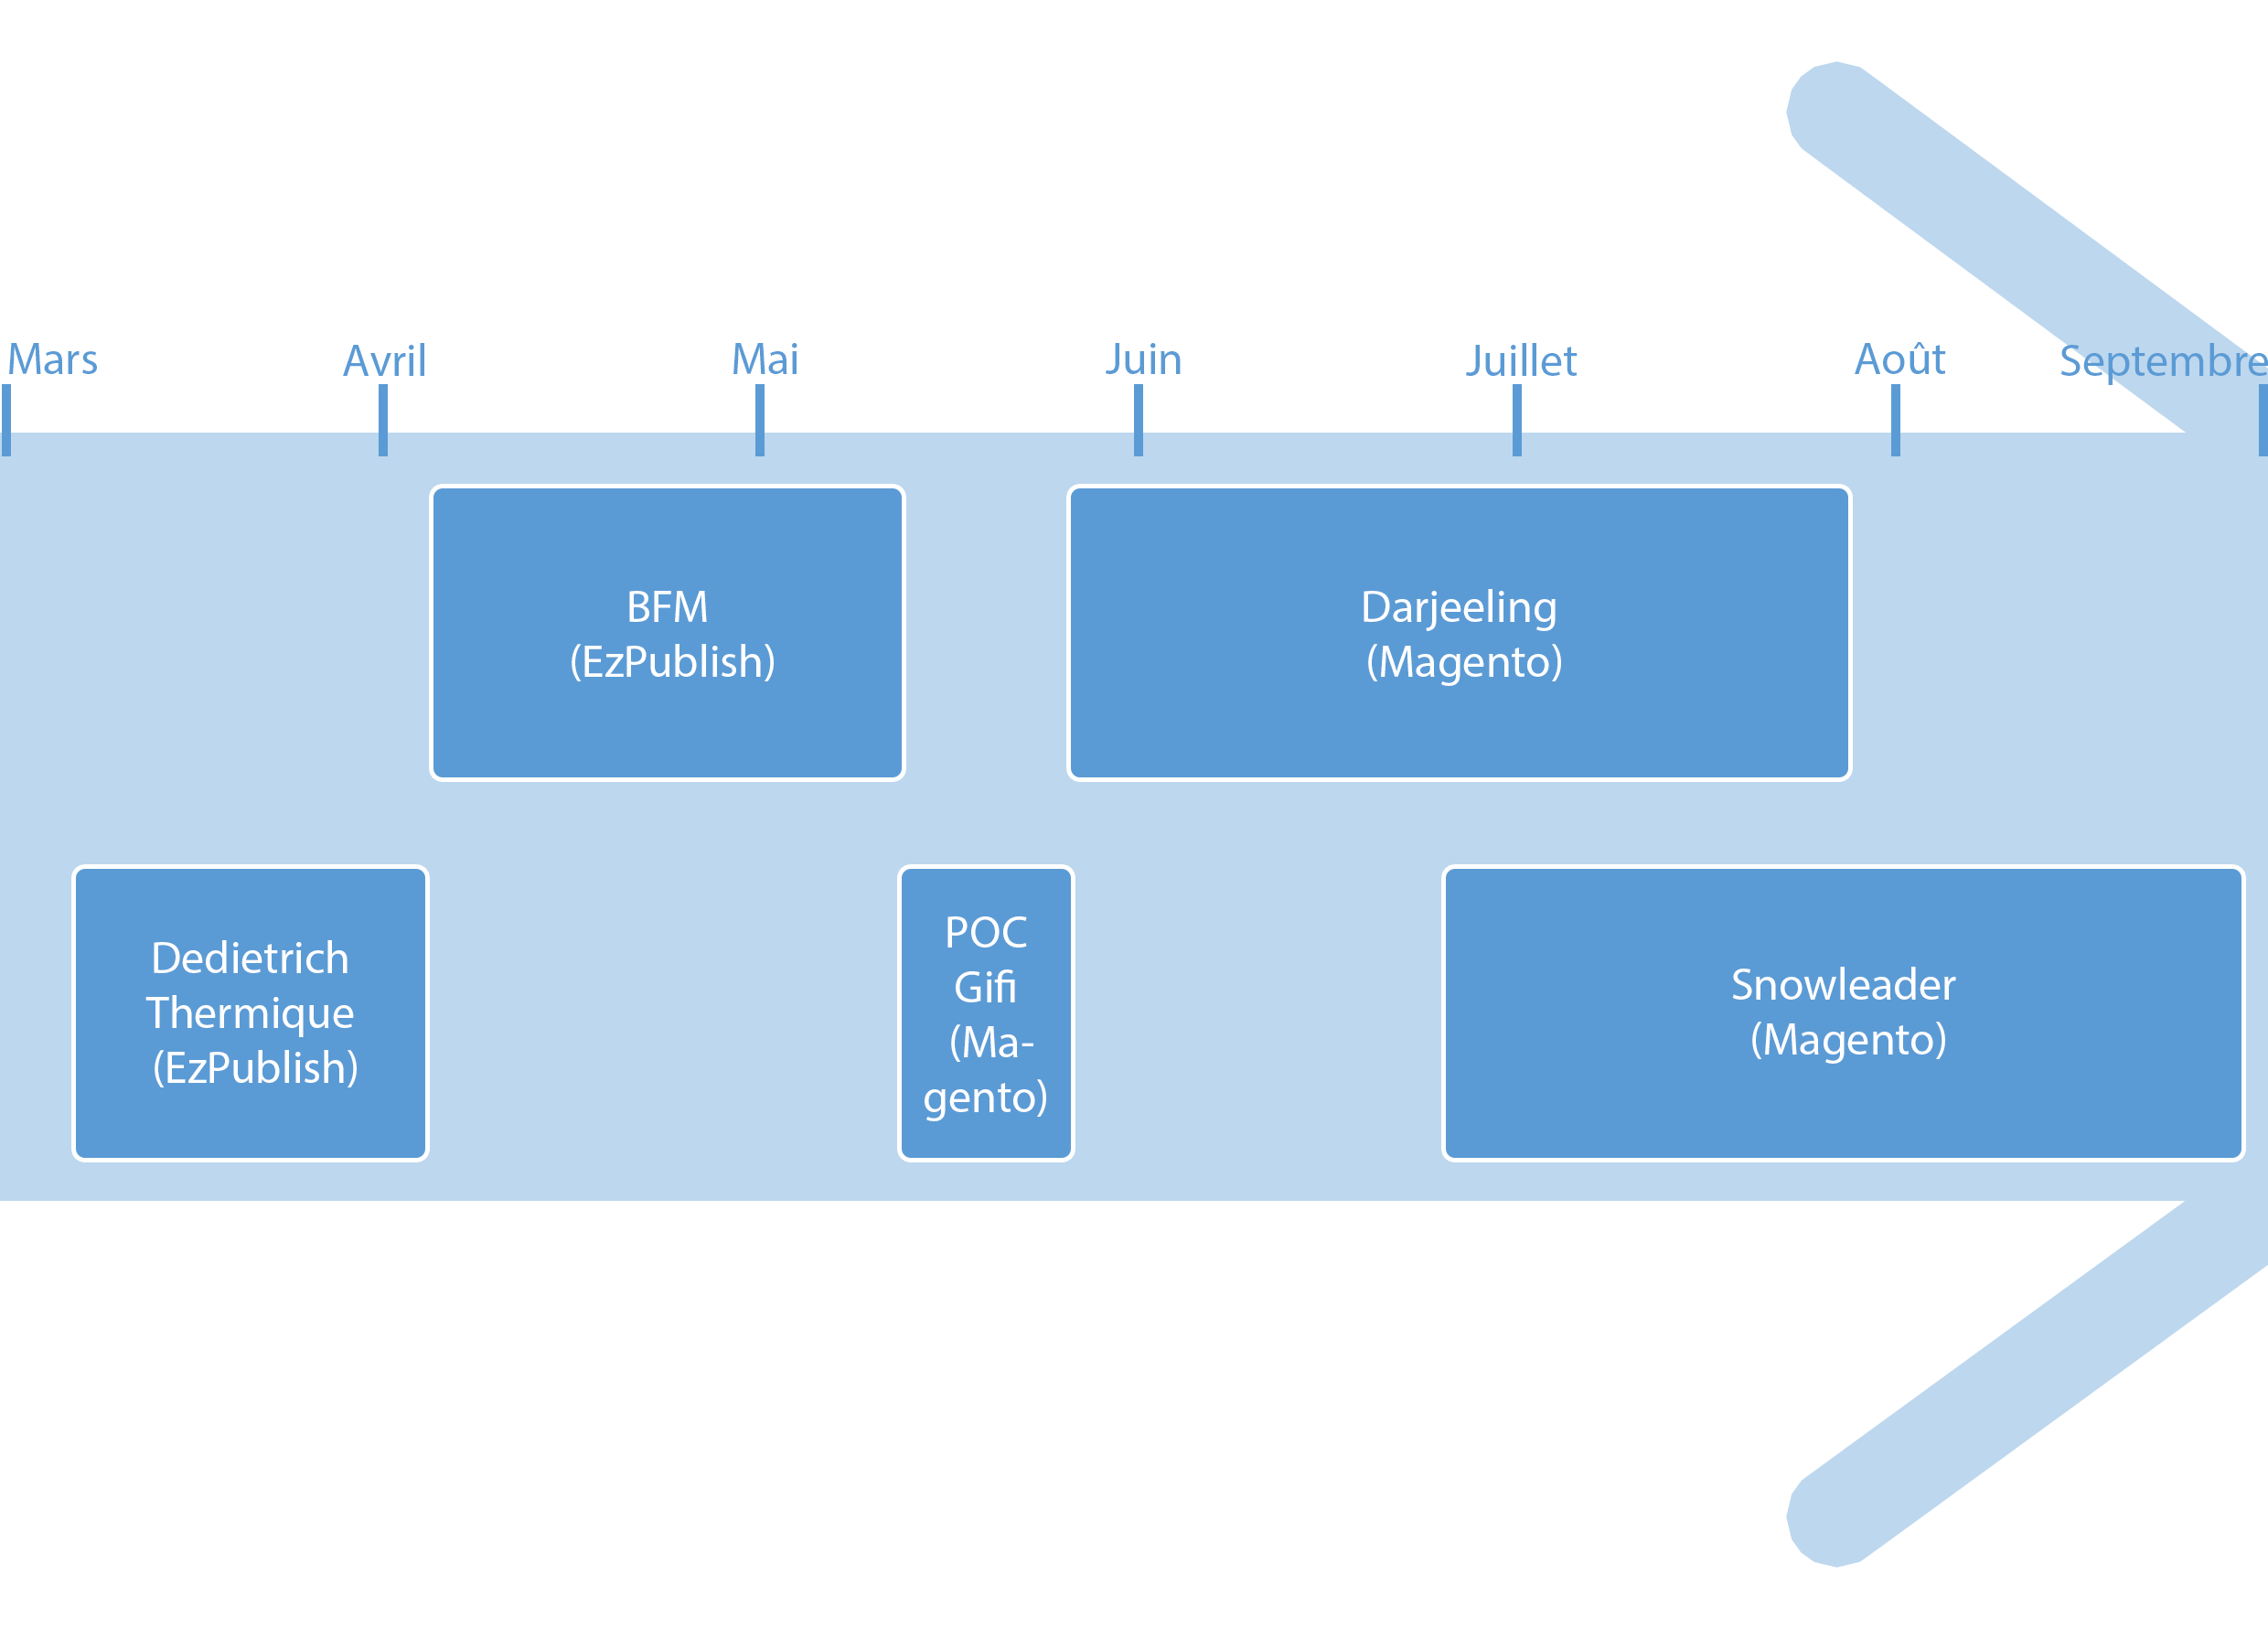
\includegraphics[width=\textwidth]{images/frise_small.png} 
	  \captionof{figure}{Chronologie de mon stage de fin d'étude chez Smile}
	  \label{frise_small}
  \end{center}
  
\chapter{Développement d'applications Web à travers différents projets}
  \section{Dedietrich thermique}
    \subsection*{Présentation du projet et état de l'art}
    \addcontentsline{toc}{subsection}{Présentation du projet et état de l'art}%Ajout de l'élément dans le sommaire
    De Dietrich est une entreprise spécialisée dans l'électroménager, le ferroviaire et le chauffage. Dans le cadre de ce projet nous travaillons sur la partie chauffage de l'entreprise, le développement du site a été réalisé avec le CMS EzPublish et plusieurs versions de ce site sont déclinées. Nous y trouvons un site principal en français \url{www.dedietrich-thermique.fr}, ainsi que des déclinaisons pour le marché russe, belge, espagnol,... A tout cela vient s'ajouter des sites mobiles eux mêmes ayant plusieurs versions en fonction des différents pays. Un service après-vente est aussi disponible en ligne et c'est dans ce cadre là que je suis intervenu. La demande du client consistait en la réalisation de sites mobiles pour leur service après-vente pour les marchés russe et belge. Ces sites existaient déjà en version française et tchèque, il fallait donc s'inspirer du travail qui avait été fait pour développer les nouveaux. 
    \subsection*{Mes objectifs}
    \addcontentsline{toc}{subsection}{Mes objectifs}%Ajout de l'élément dans le sommaire
      \begin{itemize}

	\item Mettre en place deux nouveaux sites mobiles pour les marchés russe et belge avec une version français belge et une version néerlandais belge
	\item Découvrir et prendre en main le CMS EzPublish ainsi que les méthodes de travail et de livraison propres à Smile
	\item Corriger des bugs d'affichages dûs aux différentes traductions
	\item S'assurer que les nouveaux sites créés soient compatibles avec toutes les fonctionnalités précédemment développées

      \end{itemize}
    \subsection*{Mes réalisations}
    \addcontentsline{toc}{subsection}{Mes réalisations}%Ajout de l'élément dans le sommaire
      \begin{description}

	\item[Copie de l'arborescence] J'ai commencé par copier l'arborescence des fichiers du site français déjà existant en utilisant un script développé par Smile afin de déclarer à EzPublish la création d'un nouveau site et de pouvoir l'administrer dans le back-office. J'ai ensuite modifié les fichiers de configuration du site afin d'indiquer les nouvelles URL correspondantes aux nouveaux sites ainsi que les paramètres de langues. La particularité étant la présence de plusieurs fichiers de configuration correspondant chacun à une étape du développement à savoir local, recette et production. Pour chaque cas le fichier de configuration doit correspondre au back-office de l'étape correspondante.  
	\item[Pousser en recette] Une fois mon travail réalisé et testé en local je l'ai envoyé en recette afin que le client puisse y avoir accès et puisse vérifier que cela lui convenait. Pour réaliser cette opération, là aussi des scripts ont été développés par Smile facilitant cette tâche. Ceci étant fait il reste à avertir le client via Redmine que le développement est terminé et qu'il doit nous faire des retours en vue d'éventuelles modifications à apporter.
	\begin{center}
	  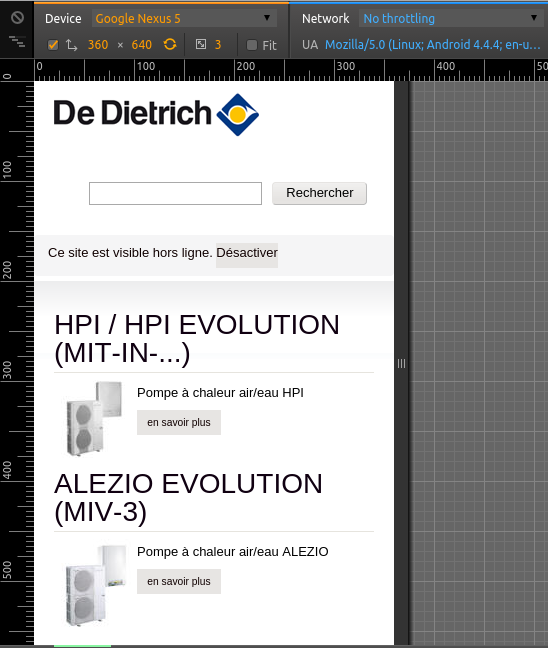
\includegraphics[width=200]{images/DDTH_home_be_fr.png} 
	  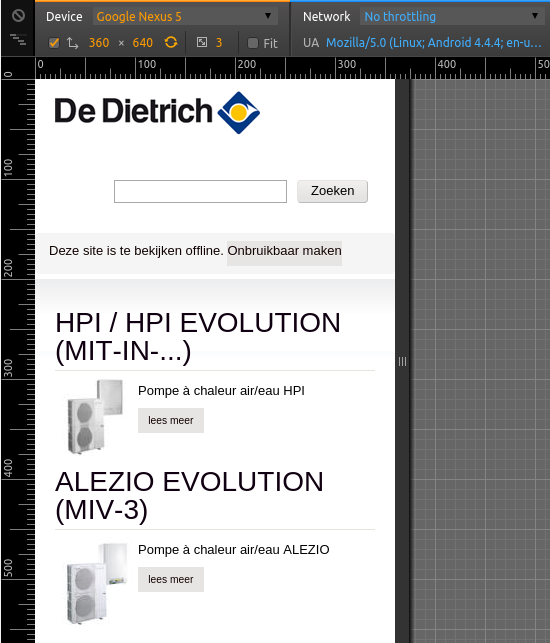
\includegraphics[width=200]{images/DDTH_home_be_nl.png} 
	  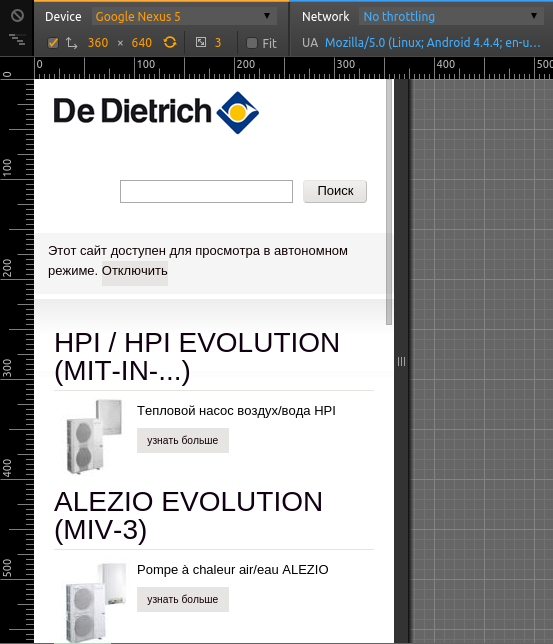
\includegraphics[width=200]{images/DDTH_home_ru.png} 
	  \captionof{figure}{Nouveaux sites mobiles (2 pour la belgique et 1 pour la russie)}
	  \label{DDTH_home}
	\end{center}
	\item[Corriger les bugs] Une grosse partie du travail consiste en la correction de bugs détectés par le client. J'ai notamment eu des modifications à apporter en terme d'affichage car les traductions dans les différents langages changent les tailles des éléments et créent des problèmes. Ceci consistait simplement en la modification des propriétés CSS pour adapter l'affichage. Des fichiers de traductions ont aussi dû être créés pour leur permettre de traduire les textes. Des fichiers pdf contenant les notices des produits ne se généraient plus sur les nouveaux sites créés, il a donc fallu modifier le code PHP pour s'adapter à ses nouveaux sites. 
	\item[Validation par le client et livraison en production] Une fois que le client a validé le travail, je suis passé à la livraison en production de la même manière que pour la recette, en utilisant un script qui facilite la chose et qui prend juste en paramètre le numéro des commits\footnote{Dans un système de gestion de version tel que SVN que nous utilisons chez Smile, la validation des modifications effectuées en local vers le serveur central est appelé un commit, qui s'accompagne généralement d'un commentaire pour expliquer les modifications apportées} à livrer. Que ce soit pour la livraison en recette ou en production il faut aussi reporter les modifications effectuées sur le back-office local vers celui de recette et de production. Une fois la livraison effectuée j'ai vérifié le bon fonctionnement du code mis en place et qu'aucun bug ne s'était glissé. Après le client peut toujours remonter un problème via Redmine, j'ai donc la responsabilité d'être à l'écoute au cas où un problème surgirait ou si une autre modification devait être apportée.  
      
      \end{description}
    \subsection*{Bilan du projet}
    \addcontentsline{toc}{subsection}{Bilan du projet}%Ajout de l'élément dans le sommaire
    Cette première participation à un projet concret fut très enrichissante aussi bien sur le plan technique qu'humain. Du point de vue technique cela m'a permis d'acquérir des connaissances sur le CMS EzPublish que je ne connaissais pas. De plus l'utilisation exclusive du terminal Linux a consolidé mes bases dans ce domaine notamment grâce à la manipulation des scripts internes à Smile que j'ai eu l'occasion de modifier moi même afin de répondre à mes besoins. En ce qui concerne EzPublish j'ai eu globalement à faire à l'ensemble des aspects du CMS ce qui m'a donné une vue générale de son fonctionnement et me permettra d'aborder les prochains projets avec plus de facilités. Quand à mes réalisations, tout s'est bien déroulé, les sites sont maintenant disponibles en ligne et le client en est satisfait. 
    
    C'est un des avantages de ce métier, c'est que l'on peut directement voir l'aboutissement de son travail une fois que celui-ci est terminé. Pour ce qui est de l'aspect humain ce premier projet m'a enseigné les méthodes de gestion au sein de Smile, tout le cheminement pour passer de la demande du client à la livraison en production. Sans oublier l'utilisation des outils internes notamment Redmine afin d'informer le client de l'avancement du développement et des problèmes rencontrés. Ainsi que la communication entre développeurs en cas de problème ou simplement pour avoir de la visibilité sur l'état du projet. Ayant que j'ai passé peu de temps sur le projet (à peine un mois), celui-ci a été très formateur et m'a permis d'appréhender la suite avec plus de facilités. C'est donc naturellement que j'ai enchaîné avec un autre projet plus long et plus compliqué, où je pourrai mettre en pratique les connaissances acquises lors de cette première expérience.  
    
\newpage
    
  \section{Banque Française Mutualiste (BFM)}
    \subsection*{Présentation du projet et état de l'art}
    \addcontentsline{toc}{subsection}{Présentation du projet et état de l'art}%Ajout de l'élément dans le sommaire
    La Banque Française Mutualiste est une banque, créée en 1986 sous le nom de Banque Fédérale Mutuelle, par les mutuelles de la Fonction publique qui ont souhaité proposer aux agents du Secteur public une banque citoyenne, qui conjuguerait les services bancaires et les valeurs mutualistes. Dans le cadre de ce projet Smile à un contrat de TMA et l'objectif est la refonte du site existant. 
    
    Dans les tâches a effectuer il y a notamment la conversion de modules anciennement en Flash vers du HTML5, l'ajout de fonctionnalités et quelques retouches graphiques. Une des possibilités intéressante est de pouvoir réaliser des simulations de prêts directement sur le site, cependant ceci est réalisé en Flash qui est une technologie propriétaire d'Adobe de moins en moins utilisée car non compatible avec les plateformes mobiles. Le client souhaitait donc redévelopper ces simulateurs en HTML5/JavaScript. De plus, ce type de simulateur est à intégrer sur d'autres sites partenaires ainsi que sur Facebook. Le problème de cette intégration est que BFM propose plusieurs types de prêts (moins de 35 ans, prêt auto, prêt travaux,...) et qu'il souhaiterait avoir un seul simulateur avec une liste déroulante permettant de choisir le type de prêt et que les taux s'adaptent en conséquence. Si sur le site de BFM avoir un simulateur de prêt par page ne posent pas de problème, il n'en est pas de même pour les sites partenaires où l'on souhaite tout intégrer dans un bloc de taille limité (notamment sur Facebook). 
    
    Parmi les nouvelles fonctionnalités que demandait le client on trouve un template vide leur permettant de créer des landing page\footnote{La landing page désigne la page sur laquelle arrive un internaute après avoir cliqué sur un lien (commercial, email, bandeau publicitaire,...). Elle a pour vocation d'être simple, belle et épurée et de transformer un simple internaute en client}, il avait l'habitude de les faire à part puis de les déposer sur le serveur, l'idée étant d'intégrer ceci au CMS EzPublish pour faciliter l'élaboration et la maintenance de ces pages. Créer un nouveau paramètre que l'on peut ajouter dans les formulaires permettant la redirection vers la page d'un produit existant tout en gardant les données déjà saisies. 
    
    Il s'agit donc d'un projet complet et complexe avec de nombreuses tâches à effectuer même si certaines se basent sur de l'existant et qu'il s'agit simplement d'un changement de technologie. Une particularité de ce projet est que nous n'avons pas accès aux serveurs de production du fait que le client soit une banque, ceci nous oblige donc à développer en interne, à leur montrer via un serveur de recette auquel ils ont accès mais pour les livraisons en production nous leur transmettons les fichiers et c'est eux mêmes qui les déploient sur leur serveur. Le principal inconvénient étant que nous n'avons pas accès au code qui est en production ce qui est parfois problématique lorsque nous n'arrivons pas à reproduire les problèmes en local. Ceci oblige à beaucoup de patience et de précision lors des livraisons et des explications pour déployer le code que nous leur fournissons.  
    \subsection*{Mes objectifs}
    \addcontentsline{toc}{subsection}{Mes objectifs}%Ajout de l'élément dans le sommaire
      \begin{itemize}

	\item Développer un simulateur de prêt en HTML5/JavaScript à intégrer sur différents sites partenaires (notamment une page Facebook), permettant la sélection du type de prêt dans une liste déroulante
	\item Convertir un simulateur d'épargne flash vers une version en HTML5/JavaScript 
	\item Développer un template intégré à EzPublish pour la création de landing page et réaliser un exemple en s'inspirant de l'existant
	\item Développer un nouvel élément de formulaire permettant la redirection vers une page produit existant et transmettant les données déjà saisies par l'utilisateur
 	\item Développer une page Web à disposition des téléconseillers intégrant une page d’orientation vers les différentes simulation de prêts personnels et une fonctionnalité d’envoi de mail type intégrant un lien vers une simulation avec des paramètres intégrés dans l’URL

      \end{itemize}
    \subsection*{Mes réalisations}
    \addcontentsline{toc}{subsection}{Mes réalisations}%Ajout de l'élément dans le sommaire
      \paragraph*{Développer un simulateur de prêt en HTML5/JavaScript à intégrer sur différents sites partenaires (notamment une page Facebook), permettant la sélection du type de prêt dans une liste déroulante}
      Pour coder cette fonctionnalité il s'agissait d'un mélange de JavaScript avec le framework jQuery et d'EzPublish. L'idée de la conception était de récupérer les différents simulateurs existant en fonction du choix de l'utilisateur dans la liste déroulante puis grâce à un appel AJAX de l'afficher. Plusieurs difficultés se présentaient à moi, récupérer le bon simulateur en fonction du choix de l'utilisateur, réussir à le charger rapidement (que ce soit transparent pour l'utilisateur) et enfin ajuster l'affichage car pour l'intégrer sur Facebook le client avait besoin du simulateur seul sans le design habituel du site. J'ai donc commencé par générer la liste déroulante en fonction des types de prêts choisis dans le back-office. En effet ce simulateur est configurable et s'adapte en fonction des types de prêts sélectionnés. Je récupère ensuite les URL correspondantes afin de pouvoir les utiliser par la suite lors de l'appel AJAX. En parallèle il a fallu créer dans le back-office la classe correspondante pour pouvoir contribuer le contenu à afficher sur les pages du CMS. C'est notamment ici que l'on décide des types de prêts qui seront proposés.
      \captionof{figure}{Récupération des données depuis le back-office et affichage de la liste déroulante}
      \label{global_loan_simulator_1}
      \lstinputlisting[language=PHP, firstline=1, lastline=18]{global_loan_simulator_1.php}
      La partie EzPublish se termine ici et il reste maintenant le JavaScript afin d'afficher le simulateur. Pour ce faire j'ai utilisé un appel AJAX qui permet l'affichage d'une page distante sans recharger entièrement la page actuelle. Pour savoir quelle page appeler on se sert de la liste déroulante et des URL récupérée précédemment. Ensuite j'ai nettoyé un peu ce qui serait affiché pour se contenter de ce qu'on avait besoin à savoir juste le simulateur.
      \captionof{figure}{Chargement en AJAX du simulateur de prêt}
      \label{global_loan_simulator_2}
      \lstinputlisting[language=HTML, firstline=1, lastline=41]{global_loan_simulator_2.html}
      Pour finir j'ai eu à adapter le style du simulateur car le client souhaitait un style différent des simulateurs habituels j'ai intégré un peu de CSS3 afin d'ajuster l'affichage. Une fois le développement terminé j'ai envoyé le lien au client pour qu'il puisse effectuer ses tests et nous faire un retour sur ce qui avait été effectué. Nous travaillions aussi avec un autre prestataire du client qui était en charge de l'intégration sur Facebook, il fallait donc aussi voir avec eux si tout était bon. Le client était satisfait et après quelques ajustements de compatibilité avec IE nous avons pu passer le simulateur en production afin de fournir l'URL final pour l'intégration d'une iframe\footnote{Une iframe est le nom d'une balise HTML qui permet d'intégrer une page HTML au sein d'un autre document HTML} sur la page Facebook. C'est à ce moment qu'un problème inattendu est arrivé car Facebook n'autorise l'intégration de lien uniquement en HTTPS or le site bfm.fr utilise HTTP, il a donc fallu développer une configuration au niveau du serveur afin de réécrire les demandes en HTTP vers HTTPS mais uniquement pour la page du simulateur que nous venions de développer car le client ne souhaitait pas que tout son site soit en HTTPS pour le moment. Une fois les tests effectués en interne nous avons pu transmettre la configuration a mettre en place sur les serveurs de production et tout était fonctionnel.
      \captionof{figure}{Configuration serveur pour la réécriture des requêtes HTTPS en HTTP}
      \label{global_loan_simulator_3}
      \lstinputlisting[language=bash, firstline=1, lastline=14]{global_loan_simulator_3.txt}
      \begin{center}
	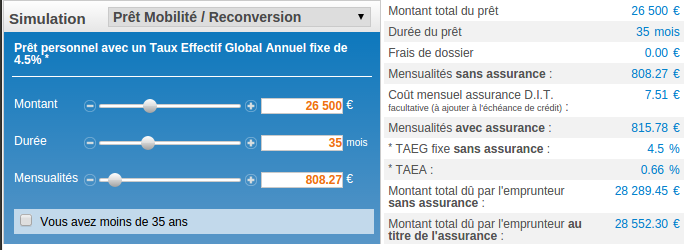
\includegraphics[width=\textwidth]{images/global_simulator1.png} 
	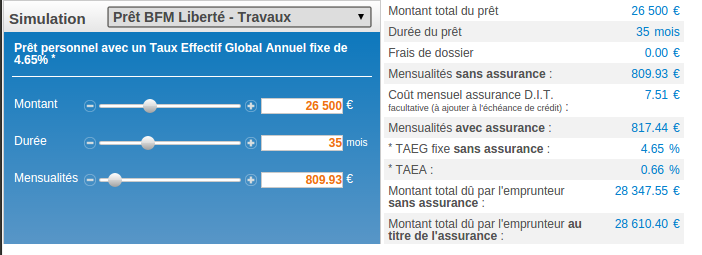
\includegraphics[width=\textwidth]{images/global_simulator2.png} 
	\captionof{figure}{Simulateur global de prêt}
	\label{global_simulator1}
      \end{center}
      \paragraph*{Convertir un simulateur d'épargne flash vers une version en HTML5/JavaScript}
      Pour développer ce simulateur j'ai pu reprendre du code existant et l'adapter aux besoins précis de ce cas. Le code est composé en majorité de JavaScript avec le framework jQuery afin d'afficher le simulateur et de traiter l'interaction avec l'utilisateur. Une partie de PHP propre à EzPublish est aussi présente afin de récupérer depuis le back-office les données choisies pour les taux d'épargnes. Ceci étant configurable j'ai là aussi créé une classe propre à ce type de simulateur et j'ai ensuite modifié le code pour récupérer les bonnes valeurs. Il n'y a pas eu de difficultés majeurs avec cette fonctionnalité car je me basais sur de l'existant il fallait donc juste faire attention à ne récupérer que le nécessaire et ensuite la partie la plus longue était d'adapter l'affichage pour ressembler à la version originale en flash, ce que j'ai réalisé en CSS (cf. Annexe Code CSS simulateur d'épargne page \pageref{code_CSS_simulateur_d_epargne}).
      \begin{center}
	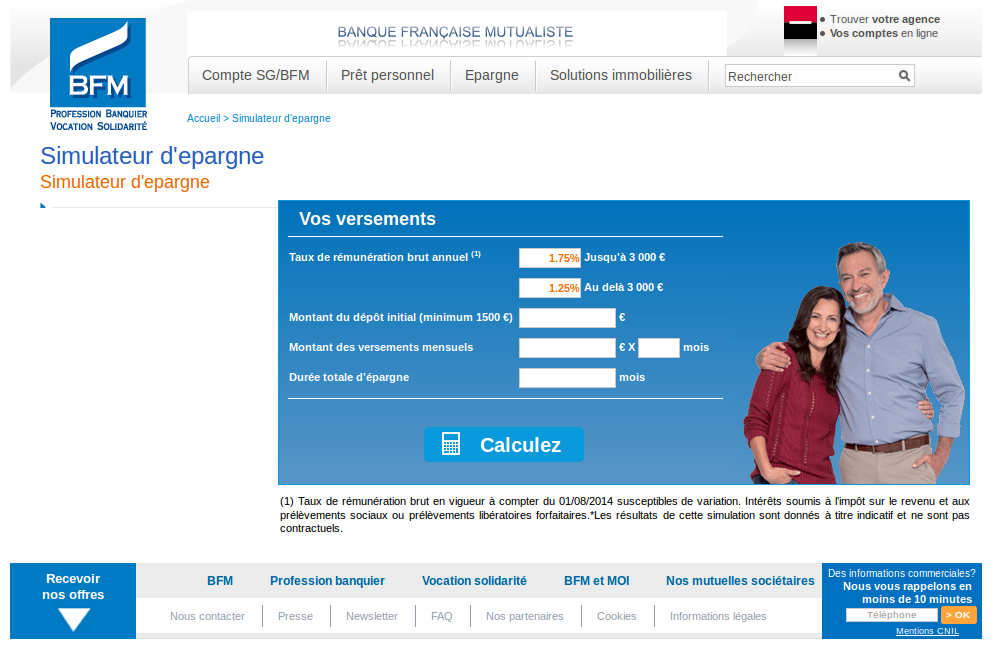
\includegraphics[width=\textwidth]{images/simu_epargne1.png} 
	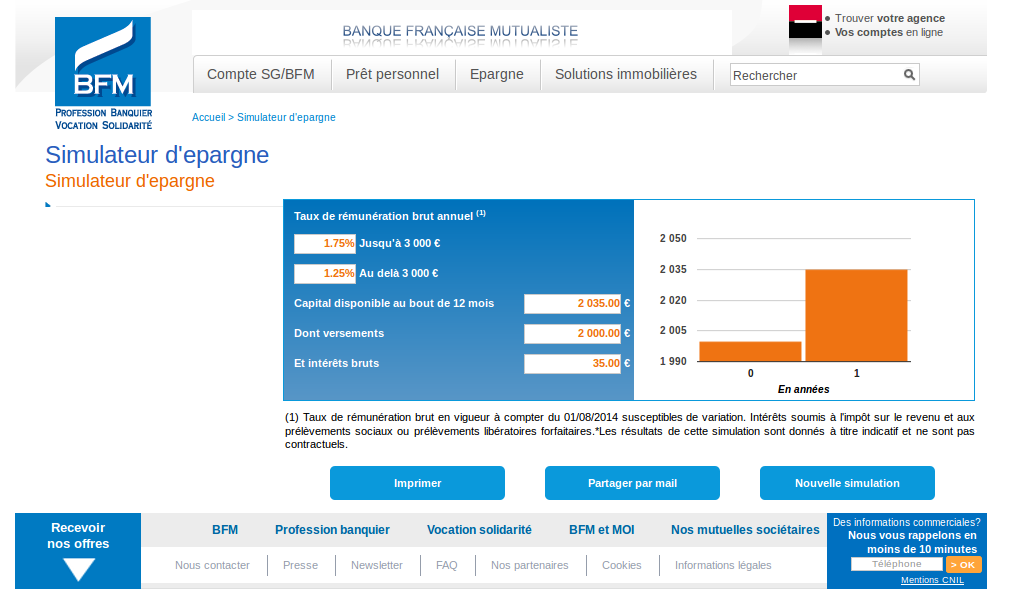
\includegraphics[width=\textwidth]{images/simu_epargne2.png} 
	\captionof{figure}{Simulateur d'épargne}
	\label{epargne_simulator}
      \end{center}
      \paragraph*{Développer un template intégré à EzPublish pour la création de landing page et réaliser un exemple en s'inspirant de l'existant}
      Dans le cadre de la création de landing page le client avait l'habitude de développer des pages à part hors du CMS puis de les déposer sur le serveur. Ceci pose problème pour la maintenance et rend la page non contribuable depuis le back-office d'EzPublish. J'ai donc commencé par créer une nouvelle classe dans EzPublish pour les landing page et j'ai ensuite codé un nouveau layout avec uniquement les entêtes de la page et la structure HTML. Le contenu de la page devant être entièrement contribuable depuis le back-office le code était assez simple et consistait juste à récupérer les données. Afin de vérifier le bon fonctionnement j'ai intégré les landing page existantes directement dans le CMS.
      \begin{center}
	
\includegraphics[width=\textwidth]{images/landing_page1.png} 
	\captionof{figure}{Landing page}
	\label{landing_page}
      \end{center}
      \paragraph*{Développer un nouvel élément de formulaire permettant la redirection vers une page produit existant et transmettant les données déjà saisies par l'utilisateur}
      Ce développement était un des plus complexes à réaliser car presque tous les éléments devaient être configurables depuis le back-office et les données capables de passer d'un formulaire à l'autre. J'ai donc commencé par créer la classe dans EzPublish avec un bouton radio oui/non afin de lancer la redirection vers un formulaire existant. Ensuite un champ pour sélectionner le formulaire vers lequel pointer et un champ pour le message à afficher lors de la redirection. 
      J'ai ensuite créé le type d'élément à ajouter dans les formulaires que j'ai nommé «Produit Existant». C'est ici que l'essentiel du code s'est écrit, l'idée étant de récupérer les questions du formulaire vers lequel on pointe puis de comparer si les champs existent aussi dans le formulaire actuel. Si tel est le cas alors je transmets les données saisies par l'utilisateur lors de la redirection si celle-ci est actionnée. 
      
      La première partie de récupération des champs existant sur le formulaire distant se fait grâce aux méthodes fournies par le CMS et on créé ainsi des champs cachés qui permettront la transmission des données. 
      \captionof{figure}{Récupération des questions existantes sur l'autre formulaire}
      \label{question_conditionnelle_1}
      \lstinputlisting[language=php, firstline=1, lastline=24]{question_conditionnelle_1.php}
      Encore une fois la deuxième partie du développement s'est effectuée en JavaScript avec le framework jQuery. Je devais récupérer les données saisies par l'utilisateur à chaque fois qu'il quittait un champ puis les transmettre dans les champs récupérés cachés du formulaire vers lequel on pointe. Ensuite on vérifie si l'utilisateur choisit l'option «Produit Existant» et si tel est le cas on affiche la popin avec le message indiquant la redirection vers le nouveau formulaire tout en transmettant les données déjà saisies (cf. Annexe Transmission de données d'un formulaire page \pageref{transmission_de_donnees_d_un_formulaire}).
      \paragraph*{Développer une page Web à disposition des téléconseillers intégrant une page d’orientation vers les différentes simulations de prêts personnels et une fonctionnalité d’envoi de mail type intégrant un lien vers une simulation avec des paramètres intégrés dans l’URL}
      Cette page se décompose en deux parties, il en sera donc de même pour le code. Dans un premier temps une section où l'on choisit le prêt que l'on souhaite puis on indique le montant et la durée de celui-ci et enfin on le simule. Ceci génère une URL avec les paramètres intégrés et ouvre une popin avec le simulateur et les valeurs choisies. Le sélecteur de prêt se génère en récupérant les données du back-office qui est configurable en choisissant les prêts à intégrer. Ensuite avec du Javascript on récupère les valeurs saisies par l'utilisateur et on concatène celles-ci à l'URL originale du simulateur pour en former une nouvelle intégrant ces paramètres. 
      \begin{center}
	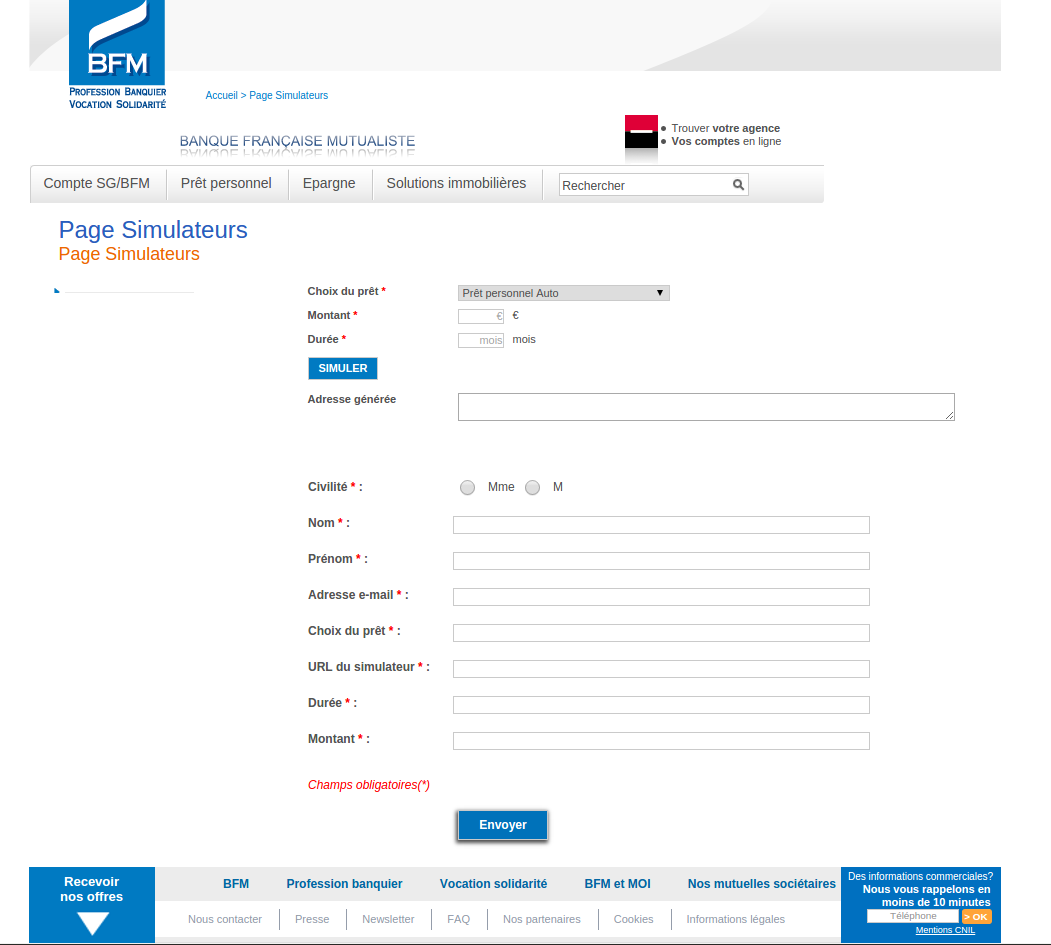
\includegraphics[width=\textwidth]{images/page_teleconseille1.png}  
	\captionof{figure}{Pages téléconseillers formulaire}
	\label{page_teleconseille_formulaire}
      \end{center}
      La deuxième section de cette page est un formulaire qui récupère toujours en JavaScript les données saisies pour la simulation plus haut ainsi que l'URL générée et permet de remplir les coordonnées du destinataire et de lui envoyer toutes les informations par mail. Ce mail devant être configurable dans le back-office et offrir la possibilité de récupérer les informations saisies par l'utilisateur et de les réintégrer dans le mail aussi bien pour l'utilisateur que pour le webmaster. 
      Nous avons rencontré des problèmes de comptabilité avec IE pour l'ouverture de la popin intégrant le simulateur, en effet le code initial était compatible avec Chrome et Firefox mais pas avec IE9 il a donc fallu le repenser afin de le rendre fonctionnel sous tous les navigateurs (cf. Annexe Illustrations pages téléconseillers page \pageref{illustrations_pages_teleconseillers}).
    \subsection*{Bilan du projet}
    \addcontentsline{toc}{subsection}{Bilan du projet}%Ajout de l'élément dans le sommaire
    Pour ce second travail avec EzPublish j'ai eu l'occasion d'exercer sur un projet d'envergure et de longue haleine. En effet BFM étant un client de TMA, de nombreuses corrections, améliorations ou évolutions sont sans cesse à apporter. Ceci offre une vraie diversité dans le projet et le rend donc très intéressant en soit mais aussi pour se former sur la technologie car il permet de couvrir une grande partie des possibilités du CMS. 
    
    D'un point de vue relationnel ce projet m'a permis d'aborder un nouvel aspect du métier d'ingénieur, à savoir la relation avec le client. J'ai été amené à plusieurs reprises à avoir des rendez-vous téléphoniques afin de discuter de l'avancement des tâches, des modifications à effectuer ou même parfois d'expliquer certains points techniques au client pour qu'il puisse configurer le site à ses souhaits. 
    
    Pour ce qui est du technique, je suis rentré véritablement dans le coeur du métier avec du PHP, du JavaScript et du style. Autant de langages peu vus en cours mais relativement simples à prendre en main que ce soit en s'inspirant de l'existant ou en recherchant sur internet. Le CMS lui aussi m'était inconnu mais j'ai pu compter sur les autres membres du projet pour m'aider et me conseiller ce qui m'a permis d'appréhender les tâches à effectuer dans de bonnes conditions. J'ai donc beaucoup appris sur ce projet que ce soit sur le plan humain ou technique, même si par la suite je vais être amené à changer de technologie et passer sur du e-commerce avec Magento, il n'en reste pas moins que les langages du WEB sont les mêmes notamment le JavaScript, CSS ou HTML et que PHP est aussi le langage serveur utilisé. 
    
    Je noterai quand même quelques difficultés rencontrées au cours de ce projet, par exemple les appels au client qui n'étaient pas simples au début par manque d'expérience dans ce domaine. Il est difficile de se mettre à la portée de la personne que nous avons au téléphone et d'être clair, précis et concis quand nous expliquons le problème rencontré ou les actions à effectuer. 
    Enfin la difficulté technique majeure de ce projet et qui à fortiori à engendrer une complication de communication, est que nous n'avions pas accès aux serveurs de productions et de pré-production comme je l'ai expliqué plus tôt. Ceci a rendu difficile les processus de livraison où le client lui même devait effectuer certaines manipulations et nous a obligé à être très précis et patient dans nos explications. Parfois nous avions des bugs que nous n'arrivions pas à reproduire en interne et nous ne pouvions pas voir ce qui se passait dans les logs\footnote{Le concept de log est l'enregistrement dans un fichier précis de certaines données ou d'événements que le développeur a besoin de connaître, sans pour autant affecter ou s'afficher sur le programme principal. Dans notre cas de site Web ce sont des données qui ne s'afficheront pas en front par exemple} rendant la tâche de debug\footnote{Action d'analyse et de correction des bugs} compliquée. De nouveau un bilan positif qui me motive pour le prochain projet en attente, avec en plus la découverte d'une nouvelle technologie, Magento.
    
    \newpage
    
  \section{POC (Proof Of Concept) thème responsive Gifi}
    \subsection*{Présentation du projet et état de l'art}
    \addcontentsline{toc}{subsection}{Présentation du projet et état de l'art}%Ajout de l'élément dans le sommaire
    L'idée de ce « mini-projet » ou POC était de vérifier la faisabilité d'un changement de thème sans modifier la version de l'application. Le site e-commerce de Gifi étant dans une ancienne version de Magento 1.13 sans thème responsive d'intégré. Nous voulions récupérer le thème responsive natif de la nouvelle version de Magento 1.14 et vérifier que sa mise en place ne casse pas le design et le fonctionnement actuel du site. 
    \subsection*{Mes objectifs}
    \addcontentsline{toc}{subsection}{Mes objectifs}%Ajout de l'élément dans le sommaire
      \begin{itemize}

	\item Intégrer le thème responsive d'un Magento 1.14 sur un Magento 1.13 

      \end{itemize}
    \subsection*{Mes réalisations}
    \addcontentsline{toc}{subsection}{Mes réalisations}%Ajout de l'élément dans le sommaire
    J'ai donc commencé par récupérer la version correspondante à celle mise en place sur le site de Gifi (Magento 1.13), je l'ai installé sur ma LXC afin de pouvoir commencer le test. Ensuite j'ai copié le thème responsive de Magento 1.14 et je l'ai chargé depuis le back-office. Il s'agissait ensuite d'effectuer des tests de compatibilité pour voir si des modules natifs de Magento ne fonctionnaient plus. Les fiches produits notamment ne s'affichaient plus correctement car une fonction n'était plus déclarée au même endroit dans le code. J'ai donc remonté ces petits bugs et confirmé la faisabilité de ce « backportage » de thème. J'en ai profité pour me former sur Magento en prévision de la formation et des projets à venir. Sachant que j'allais être amené à travailler sur le design et le templating de sites je me devais de bien assimiler la structure des pages de cette technologie. Comme on peut le voir sur le schéma ci-dessous une page est composée d'un layout qui regroupe les différents blocs et à l'intérieur de ces blocs nous avons des templates qui gèrent l'affichage. Dans ces templates on peut aussi trouver des helpers qui sont des méthodes (pouvant être issues de d'autres blocs) retournant des données.
    
    \begin{center}
      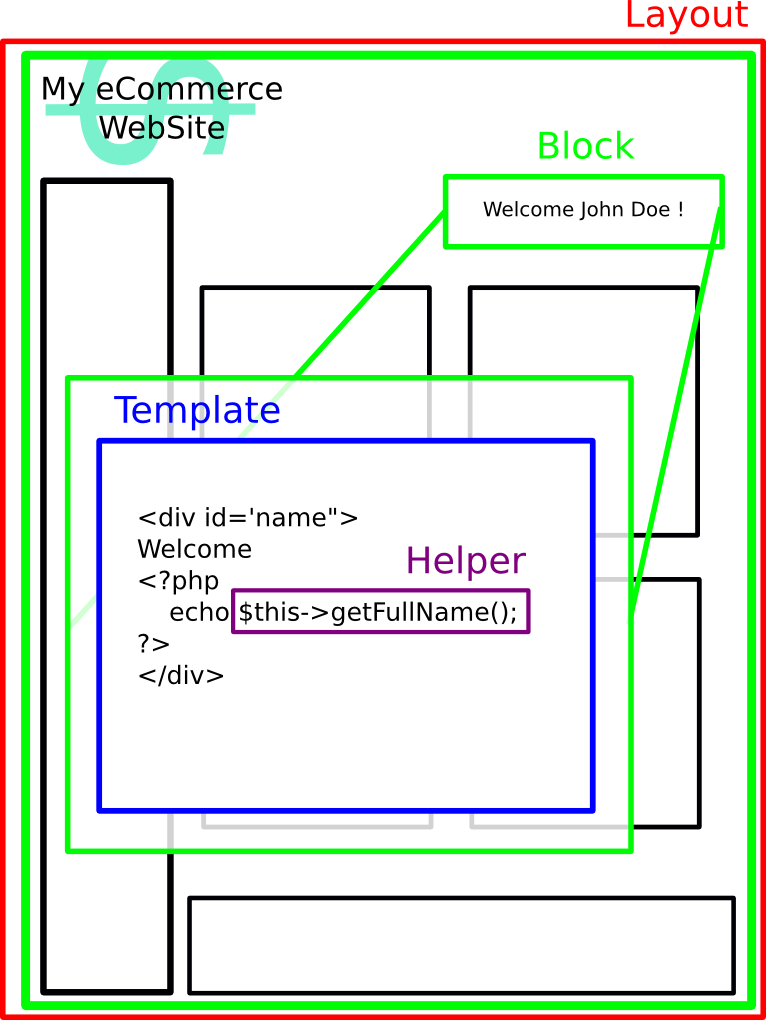
\includegraphics[width=\textwidth]{images/magento_page_design_structure.png}  
      \captionof{figure}{Structure de base d'une page Magento}
      \label{magento_page_design_structure}
    \end{center}
    
    \subsection*{Bilan du projet}
    \addcontentsline{toc}{subsection}{Bilan du projet}%Ajout de l'élément dans le sommaire
    Plus qu'un projet en tant que tel j'ai découvert par le biais de cette mission une autre facette du métier. En effet il n'est pas rare que les clients demandent ce genre d'expertise afin de savoir approximativement la faisabilité d'une évolution et surtout son coût. Car le POC a aussi pour vocation de donner un ordre d'idée du temps nécessaire à la réalisation et donc le budget à y consacrer. C'est donc un bon moyen pour le client de se rendre compte si l'investissement en vaut la peine ou s'il est préférable de se passer de ce développement et de consacrer le budget à autre chose. D'un point de vue purement technique cela m'a permis de prendre en main Magento et de bien assimiler les notions de thème, de layout et de template qui sont des aspects clés des projets où je serai amené à travailler par la suite. 
    \begin{center}
      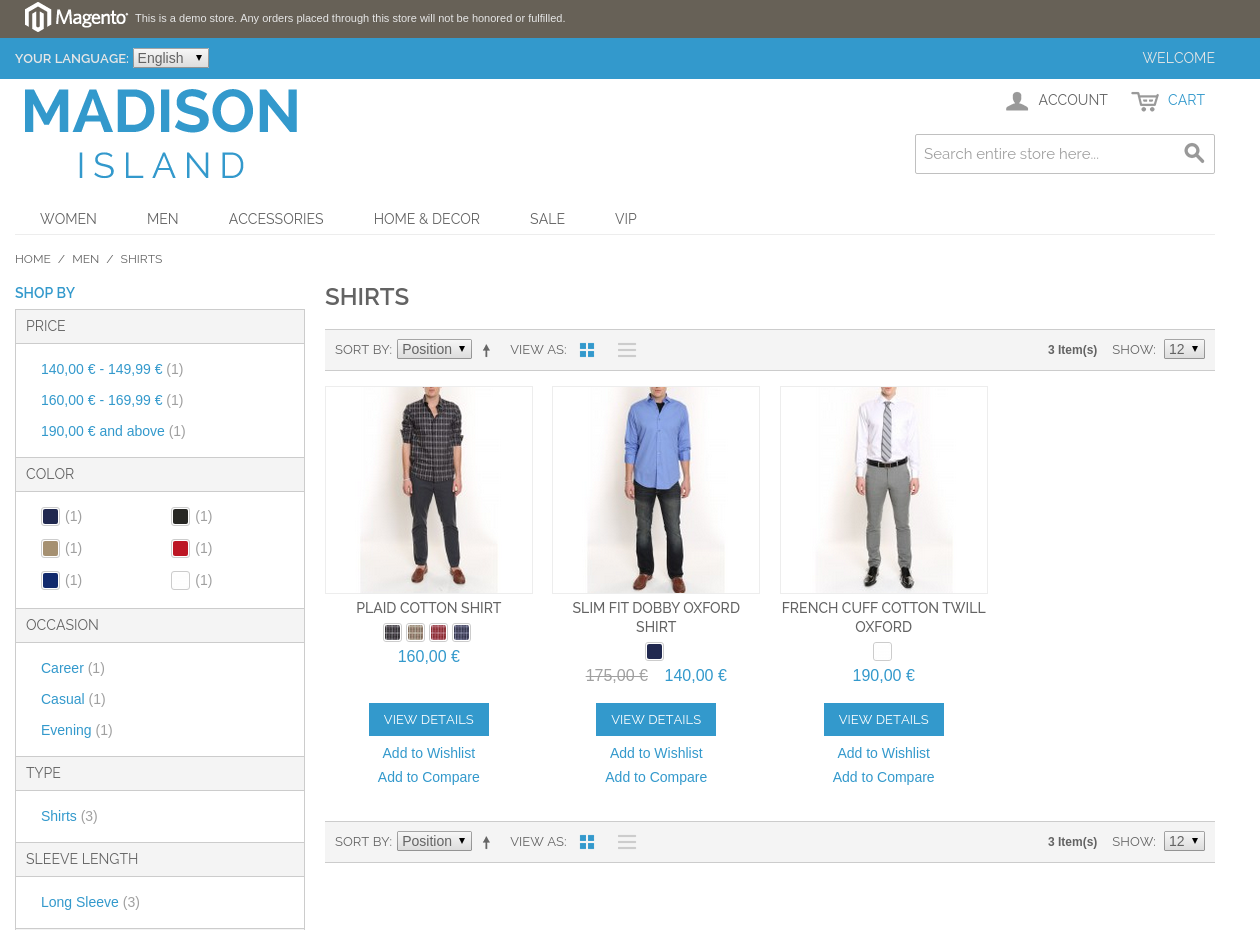
\includegraphics[width=\textwidth]{images/new_responsive_magento_theme.png} 
      \captionof{figure}{Theme responsive Magento 1.14 demo}
      \label{responsive_theme_magento}
    \end{center}

    \newpage
    
  \section{Refonte graphique Darjeeling}
    \subsection*{Présentation du projet et état de l'art}
    \addcontentsline{toc}{subsection}{Présentation du projet et état de l'art}%Ajout de l'élément dans le sommaire
    Darjeeling fait partie des clients de Smile depuis relativement longtemps, le site initial a été réalisé par le groupe. Il s'agit d'un site e-commerce de lingerie proposant de nombreux produits et les services associés, il est à noter que des magasins physiques sont présents partout en France. Aujourd'hui nous intervenons dans le cadre d'une refonte graphique et allons modifier principalement les templates, les styles et s'assurer de ne pas dégrader le résultat sur mobile. Il n'y a donc pas ou très peu de développement fonctionnel sur ce projet, uniquement du visuel. 
    
    Les technologies utilisées n'en sont pas moins intéressantes, notamment le système mis en place pour la compilation des fichiers de style et JavaScript. En effet nous utilisons Sass (Syntactically Awesome Style Sheets) qui est une sorte d'amélioration du langage CSS et qui y ajoute certaines fonctionnalités. Ces fichiers doivent être ensuite compilés pour obtenir un CSS qui est le seul langage compris par les navigateurs. Pour ce faire nous utilisons Grunt qui surveille toutes modifications apportées aux fichiers Sass et qui non seulement les compile mais les minifie aussi. Au final nous obtenons un seul et unique gros fichier CSS qui est la concaténation de tous les fichiers Sass. Ceci permet de développer sur des fichiers séparés et clairs puis de livrer au serveur un fichier unique ce qui est préférable en terme de performance. Comme la plupart des projets la principale difficulté sera le temps, car nous ne disposions que de deux mois pour réaliser le projet.
    \subsection*{Mes objectifs}
    \addcontentsline{toc}{subsection}{Mes objectifs}%Ajout de l'élément dans le sommaire
      \begin{itemize}

	\item Refonte du template et du style de divers pages du site
	\item Refonte de la liste produits et de ses filtres
	\item Optimisation du nouveau design sur mobile
	\item Phase de recette avec le client

      \end{itemize}
    \subsection*{Mes réalisations}
    \addcontentsline{toc}{subsection}{Mes réalisations}%Ajout de l'élément dans le sommaire
    	\paragraph*{Refonte du template et du style de divers pages du site}
	Il s'agit pour moi de mon premier gros projet en utilisant Magento, j'ai donc commencé par réaliser la refonte des pages les plus simples à savoir le header et le footer. J'ai donc redesigné ces pages en suivant les maquettes graphiques fournies par le client. Il y avait notamment des changements de logos, d'icônes, de couleurs et de polices mais aussi quelques modifications fonctionnelles comme le changement des liens présents dans le header et le menu de navigation (cf. Annexe Illustration footer Darjeeling page \pageref{darjeeling_header}). 
	J'ai eu par exemple à ajouter des champs dans le back-office permettant au contributeur d'ajouter une image et un lien de promotion directement dans le menu. Ceci doit être configurable, j'ai donc commencé par développer un « installer » qui permet l'ajout d'attributs dans le back-office (par modification de la base de données), un pour le choix d'une image et l'autre pour le lien vers lequel pointe cette image (cf. Annexe Installeur Magento pour ajouter un attribut au BO\footnote{Back-Office} page \pageref{installeur_Magento_pour_ajouter_un_attribut_au_BO}). J'ai ensuite modifié le template du menu afin de faire appel à ces attributs et ainsi afficher le contenu ajouté. Finalement j'ai adapté le style pour respecter la mise en forme souhaitée par le client. 
	
	\begin{center}
	  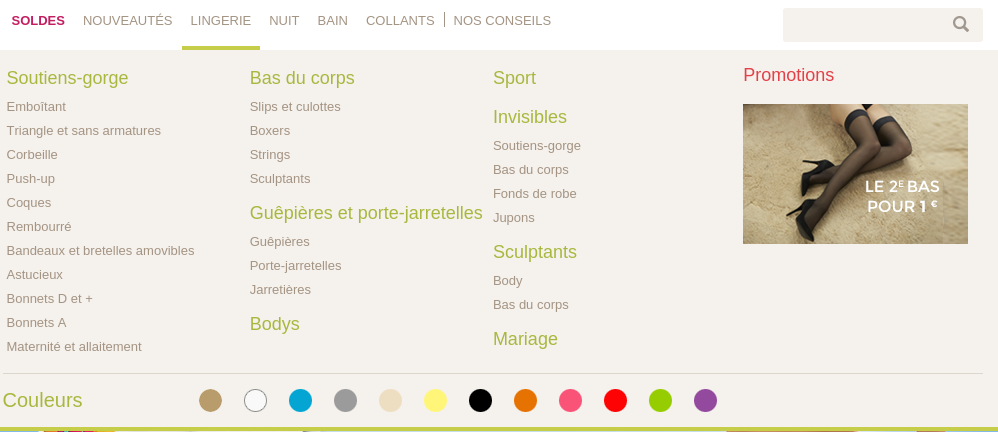
\includegraphics[width=\textwidth]{images/darjeeling_nav_menu.png} 
	  \captionof{figure}{Nouveau menu de navigation Darjeeling}
	  \label{darjeeling_nav_menu}
	\end{center}
	
	Pour le footer la partie mise en forme était assez simple, du style CSS sans complexité, la fonctionnalité intéressante réside dans la récupération des liens que l'on affiche dans celui-ci. Un attribut position avait été ajouté et je l'ai donc utilisé afin d'offrir la possibilité au contributeur de choisir dans quelle partie du footer il souhaite positionner le lien. Il ne me restait plus qu'à mettre en place une boucle dans le template qui parcourt les éléments et récupère leurs liens pour les afficher.
	\captionof{figure}{Récupération liens à afficher dans le footer depuis le back-office}
	\label{footer_recuperation_darjeeling}
	\lstinputlisting[language=html, firstline=1, lastline=19]{footer_recuperation_darjeeling.html}
	
	\begin{center}
	  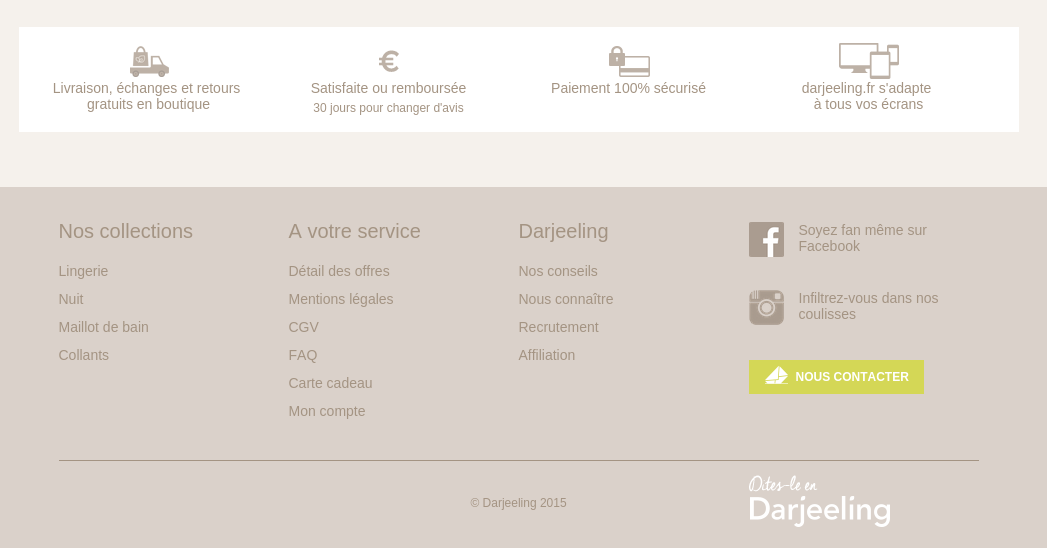
\includegraphics[width=\textwidth]{images/darjeeling_footer.png} 
	  \captionof{figure}{Footer Darjeeling}
	  \label{darjeeling_footer}
	\end{center}
	
	Par la suite j'ai réalisé la page « Mes envies » qui regroupe les produits sélectionnés par l'utilisateur et lui permet soit de les ajouter à son panier soit de les retirer de cette liste. J'ai donc redesigné la page ainsi que les blocs qui affichent les produits et implémenté un script pour l'affichage d'info bulle custom. Il s'agit uniquement de développement front, du templating et du style mais aussi du JavaScript. Sachant que cette info bulle devrait être présente à plusieurs endroits dans le site, j'ai mis en place un petit script jQuery permettant de vérifier si le produit est déjà dans la liste « Mes envies » auquel cas on propose d'enlever le produit. Dans le cas contraire l'info bulle affiche « Ajouter à mes envies ». Ce script doit être capable de réagir au clique sur le bouton et au chargement de la page, j'utilise pour cela les observeurs jQuery (cf. Annexe Script jQuery d'ajustement d'une info bulle page \pageref{script_jQuery_d_ajustement_d_une_info_bulle}).
	
	\begin{center}
	  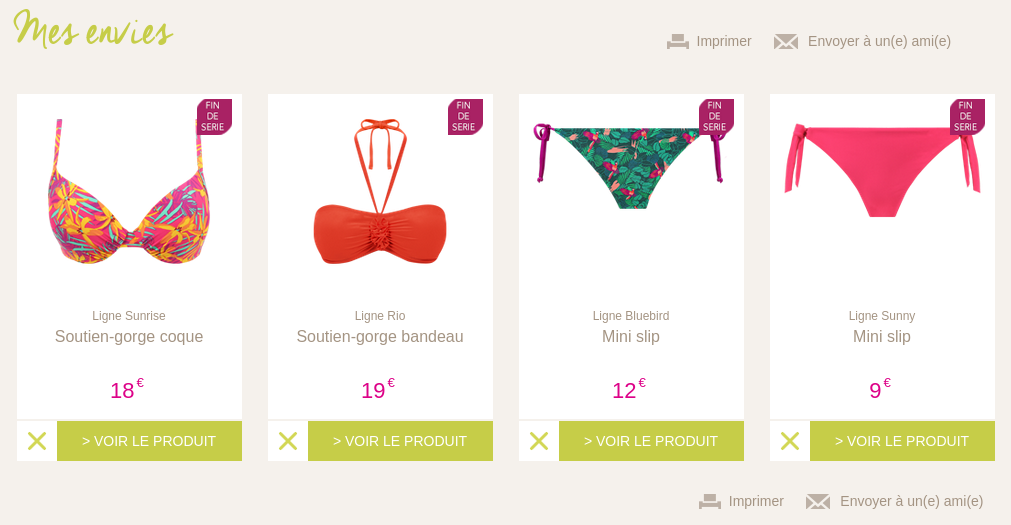
\includegraphics[width=\textwidth]{images/darjeeling_wishlist.png} 
	  \captionof{figure}{Page « Mes envies » Darjeeling}
	  \label{darjeeling_wishlist}
	\end{center}
	
	\paragraph*{Refonte de la liste produits et de ses filtres}
	La liste produits est un template appelé à différents endroits du site notamment lorsque l'on sélectionne une catégorie particulière ou que l'on effectue une recherche. Ce template est chargé de lister les produits comme son nom l'indique, de mettre en place une pagination et de proposer divers filtres pour trier les résultats. Pour ce qui est de l'affichage j'ai mis en place un nouveau design de blocs sur trois colonnes respectant les maquettes. 
	Le client souhaitait afficher 48 produits par page et proposer un lien en bas permettant de charger les 48 produits suivants. J'ai donc implémenté cette fonctionnalité par le biais d'un appel AJAX qui charge les éléments sans avoir à recharger toute la page. J'ai aussi adapté le template pour répondre à ces nouveaux besoins (cf. Annexe Illustration voir plus de produits Darjeeling page \pageref{darjeeling_see_more_products}). 
	
	\begin{center}
	  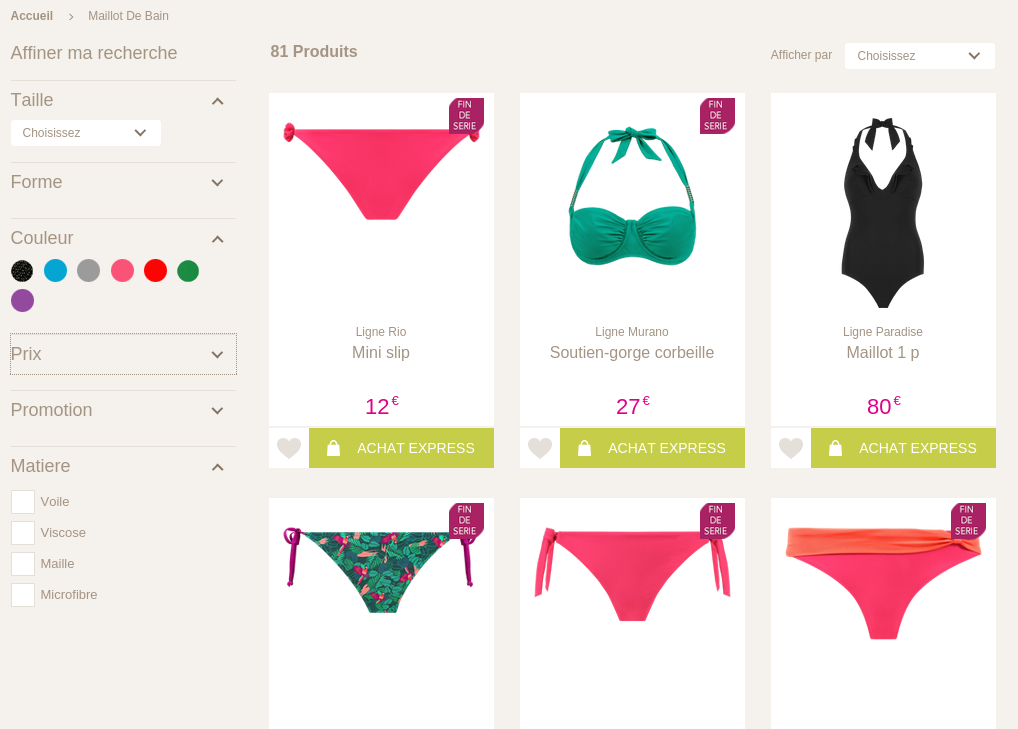
\includegraphics[width=\textwidth]{images/darjeeling_list_products.png} 
	  \captionof{figure}{Liste produits}
	  \label{darjeeling_list_products}
	\end{center}
	
	Les blocs affichant les produits ont aussi été modifiés en ajoutant de nouvelles fonctionnalités d'achat et de déplacement dans la liste de souhait. J'ai notamment utilisé le script développé et cité précédemment. 
	Concernant la partie filtre j'ai repris le fonctionnement qui était déjà en place en terme de fonctionnalités et j'ai ajouté des éléments de design en plus de la refonte graphique. Ceci s'est traduit par l'utilisation de JavaScript pour mettre en place une liste déroulante permettant d'afficher ou non le détail des filtres. Ainsi qu'un script qui regarde quelles filtres sont actifs au changement ou rechargement de la page et les réouvre directement dans le but d'améliorer l'expérience utilisateur. 
	\captionof{figure}{Script jQuery d'affichage en accordéon des filtres}
	\label{script_accordion_active}
	\lstinputlisting[language=html, firstline=1, lastline=31]{script_accordion_active.html}
	\paragraph*{Optimisation du nouveau design sur mobile}
	Le site mobile de Darjeeling venait tout juste d'être refait par Smile, il s'agissait donc juste d'impacter les principaux changements graphiques sur cette plateforme. Uniquement du développement graphique, changement de couleurs, de logos,... Enfin j'ai dû m'assurer que les changements fonctionnels sur le site desktop ne cassait pas le fonctionnement sur mobile puisque certains modules sont repris dans les deux cas. 
	\begin{center}
	  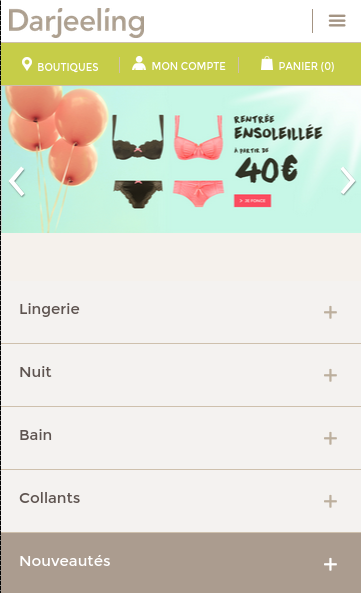
\includegraphics[width=240]{images/darjeeling_mobile_home.png} 
	  
\includegraphics[width=240]{images/darjeeling_mobile_footer.png} 
	  \captionof{figure}{Adaptation du nouveau design sur mobile}
	  \label{darjeeling_mobile}
	\end{center}
	\paragraph*{Phase de recette avec le client}
	Une fois les développements terminés nous avons passé le projet sur le serveur de préproduction afin que le client puisse regarder et tester ce qui avait été fait. L'intérêt de cette phase est d'avoir les retours du client et si une anomalie est détectée il créé un ticket sur Redmine (notre plateforme de gestion de projet) nous indiquant le problème rencontré. Celui-ci est ensuite vérifié par le chef de projet par s'assurer qu'il s'agit bien d'une anomalie rentrant dans le périmètre du projet et non une évolution à facturer en plus au client. Dans le premier cas le ticket est affecté à un développeur qui va corriger le problème puis le relivrer pour que le client puisse s'assurer que tout est réglé. 
	L'intérêt pour moi durant cette phase du projet a été de pouvoir évoluer sur l'ensemble du site et non uniquement sur le développement que j'avais effectué lors de la phase précédente. En effet j'ai été amené à corriger des bugs, apporter des modifications ou même ajouter de nouvelles fonctionnalités sur des pages qui ne me concernaient pas initialement. 
	
	Par exemple l'ajout d'un lien configurable sur un widget de la home page. Je n'avais pas travaillé avec les widget tout au long du projet et finalement, cela a été l'occasion pour moi de les découvrir. J'ai donc ajouté un attribut au widget permettant au contributeur de sélectionner si oui ou non il souhaite que le lien s'affiche. Puis dans le template ajouter une condition sur l'affichage du lien en récupérant l'information saisie dans le BO.  
    \subsection*{Bilan du projet}
    \addcontentsline{toc}{subsection}{Bilan du projet}%Ajout de l'élément dans le sommaire
    La mise en production du site à été une réussite, on peut donc dire que le projet s'est bien déroulé car l'objectif final est atteint et le client est satisfait. La période de garantie et la TMA seront là pour corriger les éventuels problèmes qui pourraient survenir. D'un point de vue personnel je suis satisfait de mes réalisations sur le projet étant donné les délais, notamment sur la phase de recette où j'ai du faire preuve de réactivité face aux retours du client. Je me suis rendu compte par le biais d'échanges avec le chef de projet qu'il était compliqué de gérer les problèmes relevés par le client. En effet il faut savoir dire non, lorsqu'un ticket relève d'une évolution et non d'une correction. La connaissance du périmètre du projet est essentielle et sa frontière parfois mince. Le temps et le budget étant limités nous ne pouvons pas tout faire sans dépasser du planning même si parfois en tant que développeur nous aimerions optimiser le rendu.
    
    Ce projet m'a énormément enseigné sur Magento grâce à la collaboration avec les autres membres du projet,ce qui m'a permis de progresser rapidement et de devenir autonome sur la plupart des tâches. J'ai ainsi pu réaliser la recette par moi même pour ce qui est des problèmes liés au design du site. J'ai eu l'occasion d'aborder certains points fonctionnels de Magento ce qui me sera utile pour la suite de mon stage et surtout j'ai acquis des méthodes de travail pour le debug. De nombreux moyens sont mis à disposition par Magento pour détecter et corriger les problèmes (notamment les logs) et j'ai appris à m'en servir efficacement. Aussi, ma compréhension de l'architecture et du fonctionnement global de cette technologie e-commerce s'est éclaircie, ainsi que les enjeux métiers relatifs au commerce sur internet.
    
    Les principaux problèmes rencontrés sont liés aux anciens développements du site, qui a été construit de manière peu conventionnel, rendant parfois notre tâche plus compliquée qu'elle ne semblait l'être. Cependant j'ai pu compter sur mes collaborateurs qui avaient de l'expérience sur le sujet pour m'aider. La seconde difficulté était le planning à tenir, celui-ci était très serré et nous a parfois obligé à faire des concessions sur la qualité du code ou sur les demandes du client. Enfin le dernier point compliqué à gérer pour moi était de mener deux projets différents en même temps car en attendant les retours de la part du client pour la recette j'ai entamé le nouveau projet sur lequel j'ai été affecté. Il a donc fallu jongler entre ces deux plateformes de e-commerce sans se mélanger ce qui était une première pour moi.   
    
        \newpage
    
  \section{Snowleader refonte 2015}
    \subsection*{Présentation du projet et état de l'art}
    \addcontentsline{toc}{subsection}{Présentation du projet et état de l'art}%Ajout de l'élément dans le sommaire
    Snowleader, c'est la référence en e-commerce pour le snow, la glisse et l'outdoor avec un catalogue de plus de 15000 références. Pour Smile Sud-Ouest cela est synonyme d'un gros projet avec de nombreuses demandes aussi bien sur le design que sur les fonctionnalités. Comme sur les autres projets nous avons des contraintes de temps bien entendu, des contraintes de performance car le catalogue est vaste ce qui fait beaucoup de données à traiter mais aussi de compatibilité. En effet le design original doit s'afficher correctement sur tous les navigateurs et être responsive sur tablette (nous ne nous occupons pas du mobile car un site à part y est dédié). 
    
    Qui dit projet conséquent, dit de nombreuses attentes de la part du client, de la précision en terme de rendu et donc une charge de travail élevée pour l'agence. C'est donc avec une équipe projet conséquente que le projet a été mené soit une dizaine de personnes, ce qui représente presque un quart des collaborateurs de Smile Sud-Ouest. Pour ma part je n'ai pas rejoint le projet dès son commencement car je travaillais sur autre chose, je suis venu en renfort au vu des besoins de développement. En effet la majorité des pages du site sont à refaire aussi bien en terme de design que d'agencement ou de fonctionnalité. Nous avons à notre disposition bon nombre de maquettes graphiques ainsi que des spécifications techniques détaillées pour nous aider dans notre travail. 
    
    Ma tâche principale est l'espace client, ce qui regroupe les pages de connexions et de déconnexions, le dashboard avec l'accès à toutes les données clients (historique de commandes, points de fidélités, ...) et les divers formulaires d'inscriptions ou de modification d'informations. 
    \subsection*{Mes objectifs}
    \addcontentsline{toc}{subsection}{Mes objectifs}%Ajout de l'élément dans le sommaire
      \begin{itemize}

	\item Refonte de l'historique des commandes et de leurs détails 
	\item Création d'une nouvelle page « Fidélités » regroupant plusieurs blocs
	\item Intégration conditionnelle de blocs CMS
	\item Gestion des informations clients

      \end{itemize}
    \subsection*{Mes réalisations}
    \addcontentsline{toc}{subsection}{Mes réalisations}%Ajout de l'élément dans le sommaire
    	\paragraph*{Refonte de l'historique des commandes et de leurs détails}
    	Nativement Magento propose aux clients un espace qui leur est réservé, un compte doit être préalablement créé par l'utilisateur pour pouvoir y accéder. Dans cet espace, il y retrouve notamment l'historique de ses commandes, passées ou en cours. Le client avait déjà redesigné cet espace lors de la version précédente, nous sommes donc loin de l'aspect natif. Cependant de nouvelles améliorations sont à apporter, en terme d'aspect, ce qui va être réalisé en suivant les maquettes graphique que nous fournient en prestataire du client. En terme de données à afficher aussi, car la nouvelle interface se veut plus épurée que l'existante (cf. Annexe Illustration dashboard Snowleader page \pageref{SL_dashboard_customer}). 
    
    	En terme de complexité, une des partie délicate a été le bouton de gauche (pentagone avec une croix à l'intérieur) que j'ai réalisé uniquement en CSS pour éviter de mettre une image et ainsi gagner en performance. Il faut en effet faire attention car le design original proposé par l'agence graphique est certes très jolie mais peut vite devenir problématique en terme de performance et d'implémentation. Pour le reste de ce tableau j'ai repris l'existant et joué avec le style car les donnés affichées sont restées les mêmes. La seule chose que j'ai ajouter c'est un lien vers une page d'impression, qui vérifie en PHP si le commande possède une facture, auquel cas le lien redirige vers la page d'impression de la facture et dans le cas contraire vers la page d'impression de la commande (cf. Annexe Condition sur le lien d'impression de facture page \pageref{SL_print_condition}).
	
	\begin{center}
	  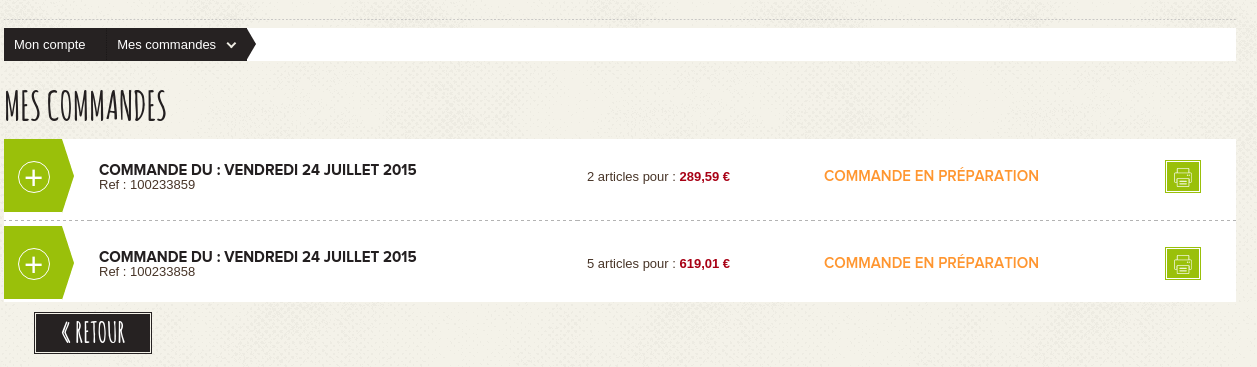
\includegraphics[width=\textwidth]{images/SL_command_history.png} 
	  \captionof{figure}{Page d'historique des commandes}
	  \label{SL_command_history}
	\end{center}
    
    	Ensuite nous rentrons dans le détail d'une commande précise, il s'agit d'une autre page, là aussi native de Magento. A l'intérieur de celle-ci nous trouvons les informations sur le client, son adresse de livraison et de facturation, les produits qui ont été commandé avec leur prix, leur quantité, ... La partie, produits commandés est restée relativement semblable au natif mise à part le style qui a été complètement revu. Là encore l'utilisation d'un tableau est le plus simple car il permet d'afficher clairement les données relatives à chaque produit. Je n'ai donc pas rencontré de difficulté majeure sur ce développement.
    
    	Sur cette même page j'ai repris la méthode développé et cité ci-dessus pour ajouter le lien vers la page d'impression avec les mêmes conditions. J'ai aussi ajouté un lien vers le suivi de la commande dans le cas où la commande a été expédiée. Pour ce faire j'utilise une méthode qui me permet de savoir si oui ou non la commande est expédiée et si tel est le cas alors je récupère son numéro de suivi que je concatène avec l'URL de suivi de colis et je l'affiche.
    
    	Grâce au BO de Magento j'ai pu tester mes différents développement, car je peux simuler depuis celui-ci le passage d'une commande puis faire avancer les étapes du processus de préparation et de livraison. Ceci m' a permis de vérifier que les diverses conditions d'affichage étaient fonctionnelles sans avoir à réellement passer de commande, ce qui me rend indépendant du reste des développements par exemple le module de paiement, le tunnel de vente, qui peuvent, eux, ne pas être fonctionnelles à l'heure actuelle (cf. Annexe Illustration back-office client Magento page \pageref{SL_BO_customer}).
	
	\begin{center}
	  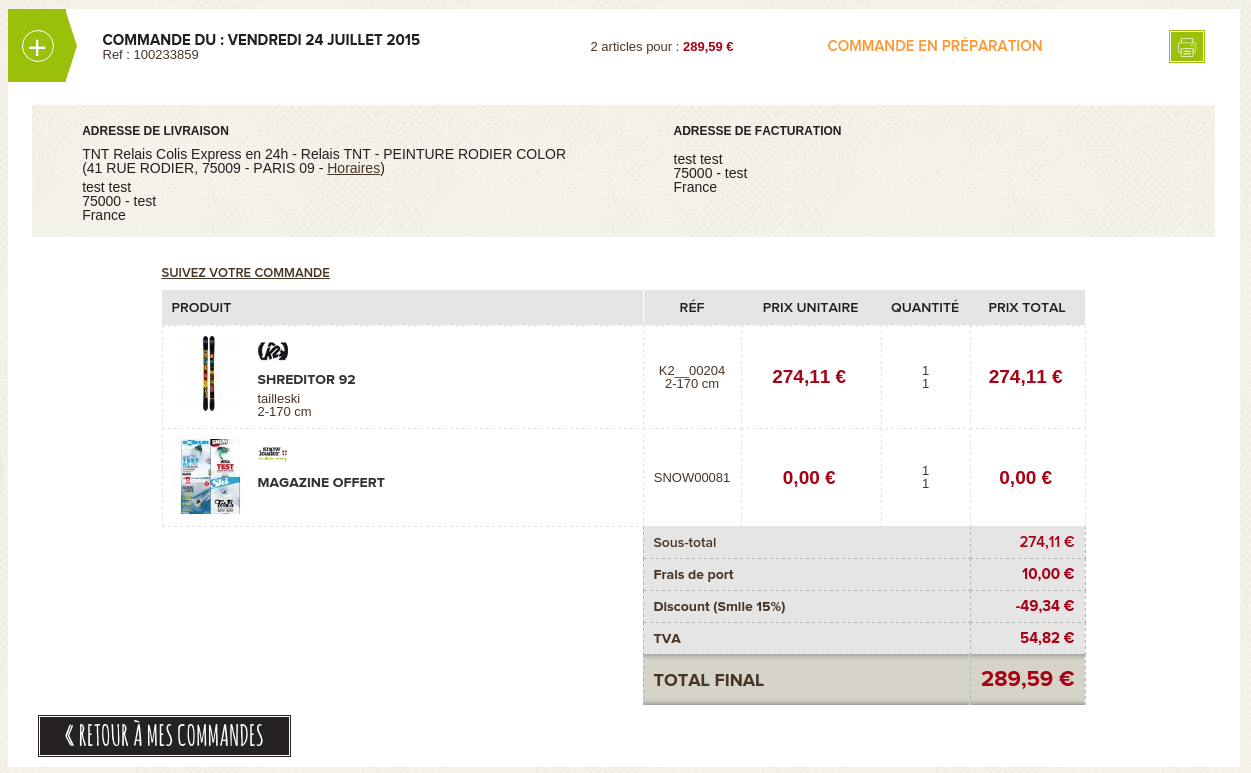
\includegraphics[width=\textwidth]{images/SL_command_detail1.png} 
	  \captionof{figure}{Détail d'une commande}
	  \label{SL_command_detail1}
	\end{center}
    	\paragraph*{Création d'une nouvelle page « Fidélité » regroupant plusieurs blocs}
    	Dans un deuxième temps j'ai eu à créer une nouvelle page qui regroupe ce qui se faisait en trois pages distinctes auparavant, à savoir, une pour les points de fidélités, une pour les crédits magasins et une pour les chèques cadeaux. Dans un soucis de facilité et d'expérience utilisateur tout rassembler en un même endroit est beaucoup plus simple et clair, cette page offre en effet la possibilité de voir ses points de fidélités et leurs historiques, de voir les crédits magasins et d'accéder à la page liée comprenant l'historique là aussi et enfin d'ajouter un chèque cadeau. On trouve en plus sur cette page un bloc CMS mais j'en reparlerai dans la partie suivante.
    
	\begin{center}
	  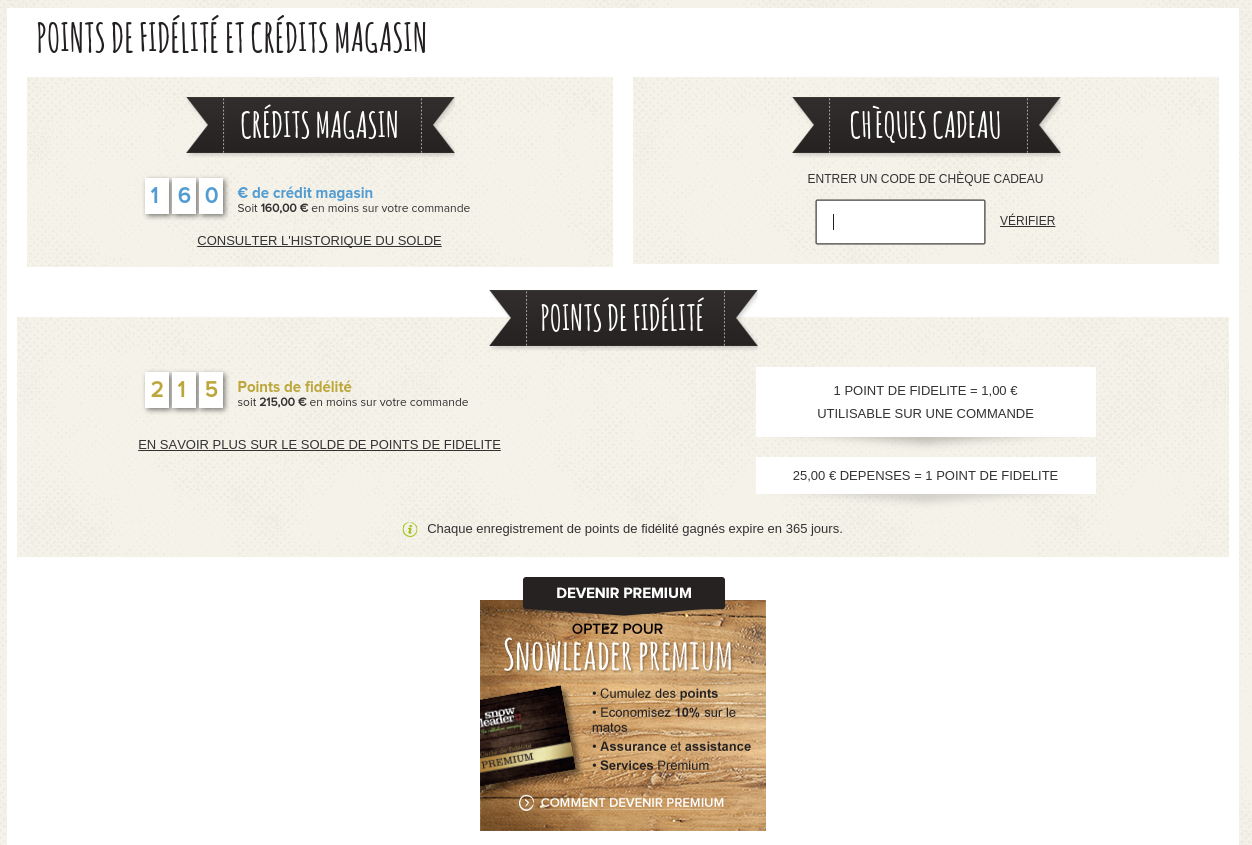
\includegraphics[width=\textwidth]{images/SL_loyalty_page1.png} 
	  \captionof{figure}{Nouvelle page Fidélité}
	  \label{SL_loyalty_page1}
	\end{center}
	
    	Je ne vais pas détaillé la création de chacune des parties de peur d'être redondant mais juste expliquer la trame générale du développement et prendre l'exemple de la partie points de fidélités. J'ai donc commencé par coder un controller capable d'intercepter l'URL customer/loyalty comme demandé dans les spécifications techniques. Pour ce faire je créé un nouveau fichier PHP dans lequel je déclare ma classe, ensuite dans la configuration du module j'ajoute un nouvel élément pour  « attraper » l'URL et utilisé la bonne classe. A cela il faut ajouter la création d'un layout custom dans lequel je déclare les blocs dont j'aurai besoin et préciser ce layout dans la configuration du module. Une fois cela terminé je me retrouve avec ma nouvelle page, mes différents blocs d'affichés provenant de l'existant, il ne me reste donc plus qu'à les modifier pour leur donner l'aspect et les fonctionnalités souhaitées (cf. Annexe Déclaration du controller custom loyalty page \pageref{SL_loyalty_controller}).
	
	Prenons l'exemple du bloc responsable des points de fidélité, dans la classe PHP de ce bloc en question je retrouve des méthodes me permettant d'effectuer diverses actions (je peux bien évidemment ajouter les miennes). A cela il faut ajouter un fichier de template pour ce bloc qui est lui responsable de l'affichage et c'est ici que nous allons retrouver la plupart du HTML ainsi qu'un peu de PHP notamment pour réaliser des boucles ou appeler les méthodes du bloc. C'est ensuite assez simple, je récupère les données dont j'ai besoin, le nombre de points de fidélités que possède le client puis je l'affiche. Cela aurait pu être aussi simple que cela mais le client avait une demande de design un peu particulière, avec une case pour chacun des chiffres du nombre. Ceci m'a obligé à développer une méthode qui sépare le nombre en chiffres puis si c'est un nombre à trois chiffres, tous les affichés, s'il n'en possède que deux ajouter un 0 avant le premier chiffre et ainsi de suite car le design comprenait trois cases.
    
    	J'ai donc créé de A à Z une page custom en allant chercher des blocs existants puis modifier le template et le style de chacun. Ceci m'a permis de voir que le potentiel de Magento est vraiment grand et que l'on peut le modifier dans le moindre détail à condition d'y mettre le temps. J'ai pu compter sur l'aide de mes collaborateurs pour m'aiguiller sur les étapes de la création et ainsi acquérir les méthodes d'experts de la technologie.
    	\paragraph*{Intégration conditionnelle de blocs CMS}
    	Une des parties du dashboard de l'espace client est composé d'une grille de blocs CMS et j'ai donc eu à la implémenter. Rien de très compliqué en soit puisqu'il m'a suffit de les contribuer dans le BO (dans un soucis de simplicité nous avons juste mis une image mais le client peut y intégrer ce qu'il veut notamment du code HTML). Puis de les déclarer dans le layout du dashboard en enfin de les appeler depuis le template. Une méthode native de Magento permet de faire cela juste en utilisant l'identifiant du bloc CMS créé dans le BO. 
	
	\captionof{figure}{Déclaration d'un layout avec l'appel à un bloc CMS}
	\label{SL_layout_custom_loyalty}
	\lstinputlisting[language=xml, firstline=1, lastline=24]{SL_layout_custom_loyalty.xml}
	
	La seule complexité à laquelle j'ai du faire face est que le client souhaitait faire apparaître un bloc différent dans deux cas, quand le client est premium et quand il est abonné à la newsletter. J'ai donc créé deux blocs CMS différents dans le BO pour chacun de ces cas. Puis j'ai codé une méthode qui vérifie si le client est premium, auquel cas grâce à une méthode native, on modifie le bloc initialement déclaré par default dans le layout et on le remplace par celui du client premium. De la même manière, j'ai créé une méthode pour les abonnés à la newsletter.
	
	\captionof{figure}{Appel du bloc CMS dans un template}
	\label{SL_block_CMS_call_in_template}
	\lstinputlisting[language=html, firstline=1, lastline=12]{SL_block_CMS_call_in_template.html}
	
	\captionof{figure}{Méthode PHP pour appeler le bon bloc CMS si le client est premium}
	\label{SL_method_to_select_CMS_block}
	\lstinputlisting[language=php, firstline=1, lastline=14]{SL_method_to_select_CMS_block.php}
		
	Le principal avantage de cette partie est de m'avoir fait prendre en main la gestion des blocs CMS qui sont souvent présents dans les différents projets car ils permettent au client de contribuer du code eux mêmes et sont donc très souple. J'ai donc appris à les intégrer et à les conditionner, mais aussi à les manipuler depuis les BO qui restait jusqu'à présent un peu flou pour moi car je ne suis pas souvent amené à le configurer.
    	\paragraph*{Gestion des informations clients}
    	Enfin ma dernière mission de développement sur ce projet a été gérer tous les formulaires que l'on peut trouver au niveau du compte client. Cela va de la popin de connection lorsque l'on est sur une page et que l'on veut se connecter ou s'inscrire, au formulaire de modification des adresses de facturation et de livraison. Je n'ai pas réinventé la roue, j'ai réutilisé les styles déjà développés en début de projet par d'autres collaborateurs. Je me suis assuré que seuls les champs nécessaires s'affichaient, que la vérifications des données côtés utilisateur et serveur s'effectuaient bien et enfin harmoniser le style des pages car elles n'étaient pas toutes présentes dans les maquettes graphiques (cf. Annexe Illustration formulaire de modification des informations personnelles page \pageref{SL_account_information_form}).
	
	J'ai eu l'occasion de refaire des scripts JavaScript et Prototype (un autre framework JavaScript utilisé sur Magento par default). Mon expérience passée sur les autres projets avec ce langage m'ont permis d'être efficace sur ce sujet ce qui m'a laissé du temps pour peaufiner le style des formulaires. 
	
	\begin{center}
	  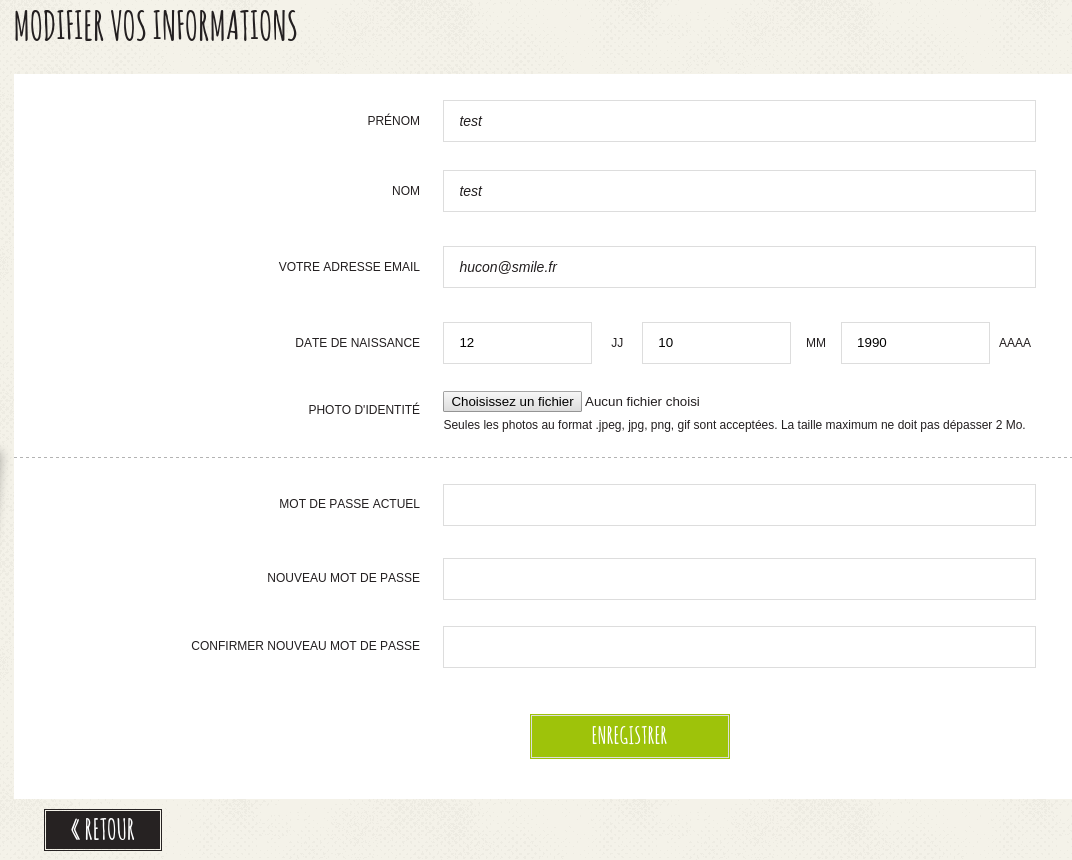
\includegraphics[width=\textwidth]{images/SL_account_information_form.png} 
	  \captionof{figure}{Formulaire de modification des informations client}
	  \label{SL_account_information_form}
	\end{center}
    \subsection*{Bilan du projet}
    \addcontentsline{toc}{subsection}{Bilan du projet}%Ajout de l'élément dans le sommaire
    Ce dernier projet fait vraiment office de bilan pour mon stage car il m'as permis de réutiliser toutes les connaissances techniques acquises au cours de ces six mois. En plus j'ai pu apprendre et utiliser des fonctionnalités plus avancés de Magento, donc j'ai encore une fois continuer d'enrichir mon bagage techniques dans le domaine du développement Web. Le fait qu'il s'agisse d'un gros projet m'a donné l'occasion d'être plus indépendant sur la partie du site qu'il m'acquittait de développer. Bien entendu je pouvais tout de même compter sur les autres membres du projet pour venir me conseiller en cas de difficulté.
    
    Le fait d'arriver en cours de projet a finalement été intéressant car cela m'a obligé à bien communiquer avec le reste de l'équipe pour être sûr de ne pas réinventer la roue mais plutôt de réutiliser d'éventuels codes déjà réalisé précédemment. De plus le chef de projet réalise des réunions d'équipe régulièrement ce qui permet non seulement de savoir où en est l'avancement du projet mais aussi d'être au courant de la répartition des tâches au différents membres du projet. Ainsi lorsque l'on a une question sur un sujet on sait rapidement à qui s'adresser. 
    
    A l'heure où j'écris ces lignes le projet n'est pas encore fini mais il est en bonne voie et devrait être livrer avec deux semaines de retard. En effet, pour diverses raison l'avancement a pris du retard et les responsables du projet en accord avec le client ont décidé de reculer la date de livraison. Encore une fois la principale difficulté est donc, le temps. Pour ma part cette « pression » de planning m'a obligé à être encore plus efficace mais c'est une des réalités du métier il est donc intéressant d'y faire face. 
    
    Finalement un des intérêts principal de ce projet a été la réalisation de code de qualité et indépendant, associé à une bonne documentation. Ceci permet aux autres collaborateurs de récupérer le code si besoin et donc de gagner un temps précieux. Afin de vérifier la qualité du code, le chef de projet technique a mis en place un système que l'on intègre à notre IDE et qui vérifie en temps réel que notre code respecte les conventions fixées (indentation, retour à la ligne, commentaires, ...). Ce chef de projet étant un expert sur la technologie, il vérifie régulièrement le code commité et peu nous faire des retours personnalisés quand à la qualité et l'efficacité de notre code. Ce qui se traduit par une progression au niveau de ma connaissance et ma maitrise de Magento. 
    
\chapter*{Conclusion}
\addcontentsline{toc}{chapter}{Conclusion}%Ajout de l'élément dans le sommaire
  \section*{Enseignements et bénéfices}
  \addcontentsline{toc}{section}{Enseignements et bénéfices}%Ajout de l'élément dans le sommaire
  Etant issue d'une formation au coeur de métier différent que celui dans lequel j'ai réalisé mon stage, j'ai pris un certain risque avec ce choix. Cependant je savais qu'il s'agissait d'un domaine qui m'intéressait et que je pratiquais déjà en dehors sur mon temps libre. En SRC et tout au cours de l'enseignement à l'INSA j'ai eu de nombreuses heures de programmation dans divers langages et appliqués à divers domaines. Fort heureusement les bases et la logique reste là même tout le temps ce qui m'a permis de m'adapter et d'apprendre rapidement. C'est donc sans regret que je me suis ouvert au domaine du développement Web.
  
  Le fait d'avoir effectué ce stage m'a évidemment permis d'acquérir de nombreuses connaissances techniques et humaines, mais encore plus du fait que celui-ci se soit réalisé dans une entreprise d'un autre secteur. J'ai de nombreuses occasions de me former, que ce soit par moi même, au cours des formations proposées par l'entreprise et surtout grâce au partage entre collaborateur. La notion de travail d'équipe autour d'un projet a véritablement pris tout son sens pendant ce stage, notamment au cours des gros projets sur lesquels j'ai été amené à travailler. Bien que nous ayons eu l'occasion d'effectuer des projets à plusieurs à l'école, le faire en entreprise apporte une autre dimension et qui permet d'acquérir une expérience très enrichissante pour notre carrière professionnelle.
  
  Bien entendu tout n'a pas été rose durant ces six mois, il a fallu apprendre à gérer la pression du planning sur les projets. J'ai rapidement compris que le temps était en quelque sorte notre pire ennemi en entreprise surtout qu'il est obligatoirement lié à des contraintes budgétaires. La notion de budget est-elle aussi importante et nouvelle pour nous qui venons du milieu scolaire. Il faut forcément la prendre en considération lorsque nous développons quitte à parfois se limiter en terme de performance et de qualité de code lorsque le budget ne le permet plus. Comme toutes les entreprises, Smile cherche à générer des profits, on ne peut donc pas aller au delà des ressources budgétaires fournies pas le client.
  
  J'ai finalement apprécié de ne pas me consacrer à un seul et même gros projet, au contraire, commencer par de plus petites missions m'a donné l'occasion d'apprendre avec des tâches plus simples et ainsi ne pas me retrouver face à une difficulté insurmontable. Cela aurait été problématique et aurait ralenti les gros projets sur lesquels j'ai été amené à travailler si je n'avais eu aucune expérience sur la technologie en question. De plus l'ensemble des projets que m'a proposé Smile étaient intéressants et variés. Ils touchaient tous à des secteurs diamétralement différents et c'est là aussi un avantage du secteur du Web (de part l'implantation des sites internet dans le monde professionnel), pouvoir proposer des sujets divers et variés en fonction des clients.
  
  Enfin je pense avoir su apporter ma polyvalence acquise tout au long de ma formation, ce qui fait que la collaboration avec les autres collaborateurs s'es très bien déroulée. Sur le plan technique j'ai beaucoup appris bien évidemment mais j'ai aussi tiré parti de mes autres expériences dans le monde professionnel et de mon enseignement à l'INSA. Notamment dans la manière de gérer des grosses charges de travail, de bien répartir son temps et de savoir être concentré, précis et appliqué lorsque l'on a un projet à mener.
  \section*{Les projets à venir}
  \addcontentsline{toc}{section}{Les projets à venir}%Ajout de l'élément dans le sommaire
  Pour ce qui est de l'avenir chez Smile Sud-Ouest, ce sont des projets toujours plus gros, par exemple la refonte du site des Taxis G7 en full Symfony 2. Il en est de même pour tout le groupe qui se voit confier des projets plus important en taille obligeant donc l'entreprise a recruter. On constate aussi que la plupart, pour ne pas dire toutes, les technologies utilisées chez Smile convergent. Que ce soit Magento, Drupal, EzPublish, toutes vont passer à un core en Symfony 2 sur leurs nouvelles versions. Selon moi et l'entreprise visiblement aussi, ce framework PHP (qui plus est français), va devenir incontournable pour le Web et va donc en quelques sortes facilité les développements. Je m'explique, un développeur connaissant Symfony 2 sera à même de coder sur Magento, Drupal, EzPublish ou en full Symfony 2 car tous seront basés sur la même architecture. Bien entendu les contraintes métiers ne seront pas les mêmes, mais d'un point de vu technique on observe une convergence intéressante. Je pense donc que beaucoup de projets utilisant ce framework sont à venir et qu'il va devenir un bagage indispensable pour les développeurs Web.
  
  En ce qui me concerne, j'ai pris conscience que le développement informatique quel qu'il soit m'intéressait. J'affectionne tout particulièrement le secteur du Web mais je ne souhaite pas me fermer des portes, c'est pourquoi je vais continuer à la suite de mon stage dans une autre SSII non spécialisé dans le Web afin de m'ouvrir encore à d'autres domaines et donc d'autres technologies. Ce stage de fin d'étude a été pour moi une très bonne expérience, aussi bien sur le plan professionnel que personnel. J'espère donc que ce nouveau travail qui m'attend continuera d'assouvir ma soif d'apprendre tout en restant réceptifs aux nouvelles technologies.
\chapter*{Annexes}
\thispagestyle{\chead{}}
\addcontentsline{toc}{chapter}{Annexes}%Ajout de l'élément dans le sommaire
  
  \section*{Annexe Code CSS simulateur d'épargne}
  \addcontentsline{toc}{section}{Annexe Code CSS simulateur d'épargne}%Ajout de l'élément dans le sommaire
  \label{code_CSS_simulateur_d_epargne}
  \lstinputlisting[language=HTML, firstline=1, lastline=68]{saving_simulator_html5.html}
  \captionof{figure}{Code CSS simulateur d'épargne}
  
    \newpage
  
  \section*{Annexe Transmission de données d'un formulaire}
  \addcontentsline{toc}{section}{Annexe Transmission de données d'un formulaire}%Ajout de l'élément dans le sommaire
  \label{transmission_de_donnees_d_un_formulaire}
  \lstinputlisting[language=HTML, firstline=1, lastline=63]{question_conditionnelle_2.html}
  \captionof{figure}{Transmission de données d'un formulaire}
  
    \newpage
  
  \section*{Annexe Illustrations pages téléconseillers}
  \addcontentsline{toc}{section}{Annexe Illustrations pages téléconseillers}%Ajout de l'élément dans le sommaire
  \label{illustrations_pages_teleconseillers}
  \begin{center}
      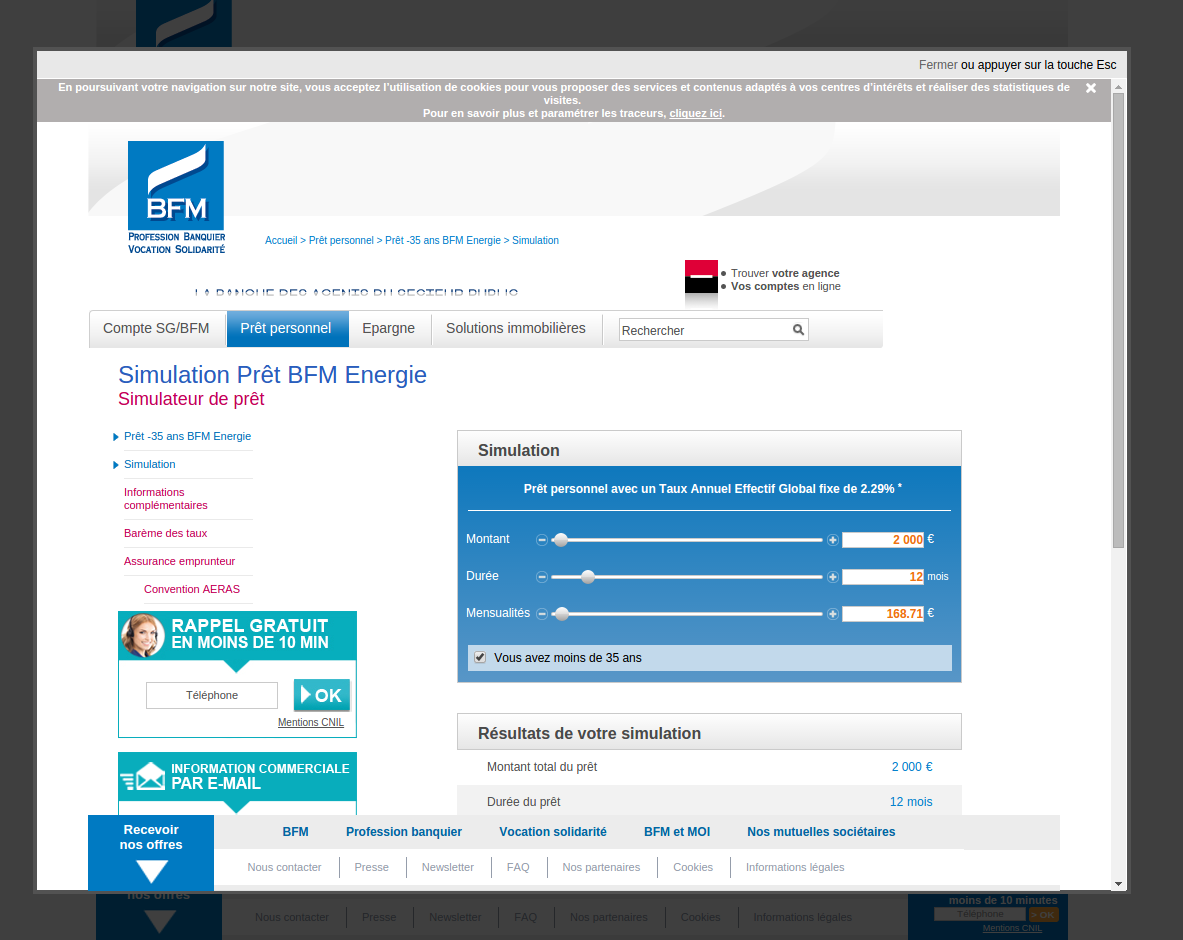
\includegraphics[width=\textwidth]{images/page_teleconseille2.png} 
      \captionof{figure}{Pages téléconseillers popin simulation}
      \label{page_teleconseille_popin_simulation}
  \end{center}
  \begin{center}
    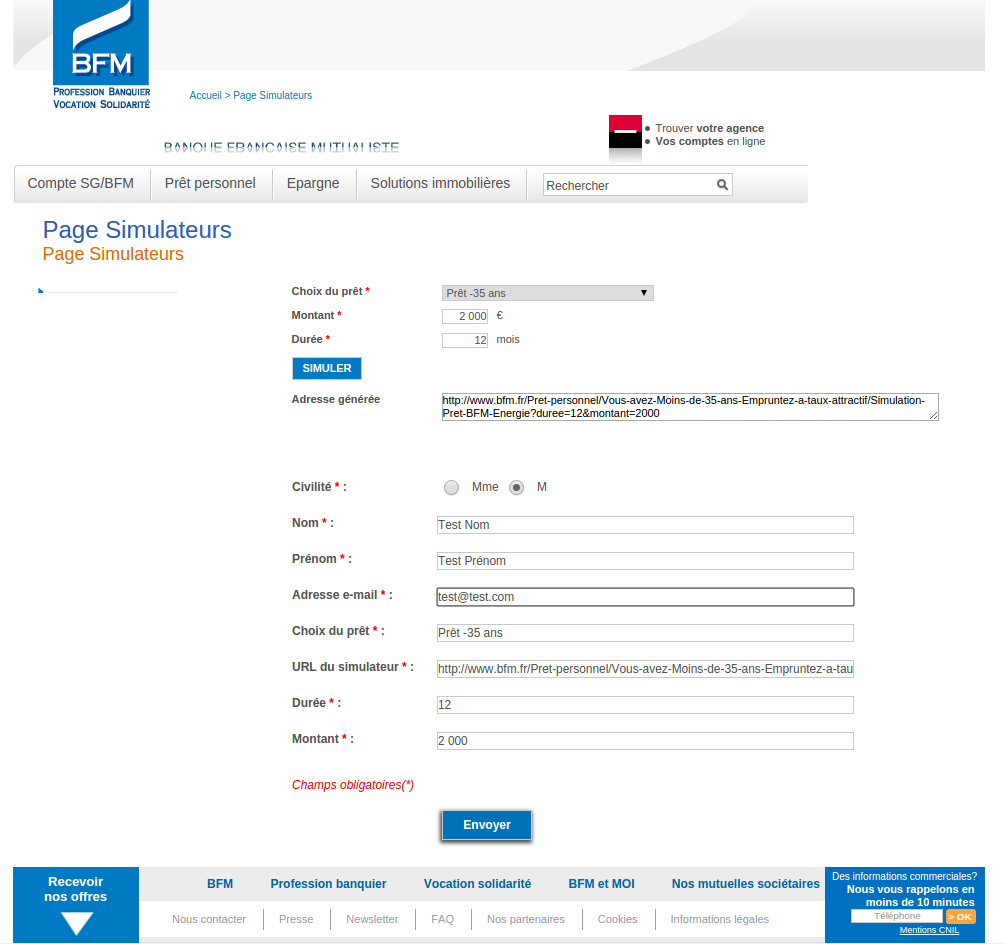
\includegraphics[width=\textwidth]{images/page_teleconseille3.png} 
    \captionof{figure}{Pages téléconseillers formulaire préremplie}
    \label{page_teleconseille_formulaire_prerempli}
  \end{center}
  
    \newpage
    
  \section*{Annexe Illustration header Darjeeling}
  \addcontentsline{toc}{section}{Annexe Illustration header Darjeeling}%Ajout de l'élément dans le sommaire
  \begin{center}
      
\includegraphics[width=\textwidth]{images/darjeeling_header.png} 
      \captionof{figure}{Header Darjeeling}
      \label{darjeeling_header}
  \end{center}
  
    \newpage
    
  \section*{Annexe Installeur Magento pour ajouter un attribut au BO}
  \addcontentsline{toc}{section}{Annexe Installeur Magento pour ajouter un attribut au BO}%Ajout de l'élément dans le sommaire
  \label{installeur_Magento_pour_ajouter_un_attribut_au_BO}
  \lstinputlisting[language=php, firstline=1, lastline=51]{installer_darjeeling.php}
  \captionof{figure}{Installeur Magento pour ajouter un attribut au BO}
  
    \newpage
  
  \section*{Annexe Script jQuery d'ajustement d'une info bulle}
  \addcontentsline{toc}{section}{Annexe Script jQuery d'ajustement d'une info bulle}%Ajout de l'élément dans le sommaire
  \label{script_jQuery_d_ajustement_d_une_info_bulle}
  \lstinputlisting[language=html, firstline=1, lastline=31]{script_tooltip.html}
  \captionof{figure}{Script jQuery d'ajustement d'une info bulle}
  
  \newpage
  
  \section*{Annexe Illustration voir plus de produits Darjeeling}
  \addcontentsline{toc}{section}{Annexe Illustration voir plus de produits Darjeeling}%Ajout de l'élément dans le sommaire
  \begin{center}
      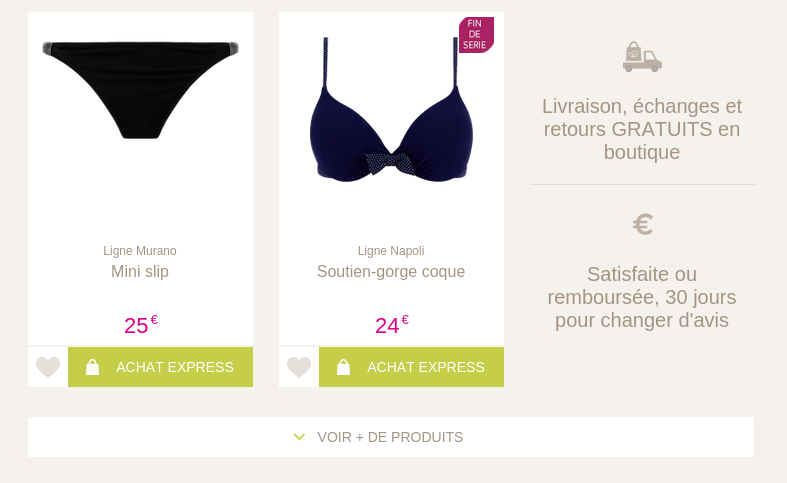
\includegraphics[width=\textwidth]{images/darjeeling_see_more_products.png} 
      \captionof{figure}{Bloc pour voir plus de produits}
      \label{darjeeling_see_more_products}
  \end{center}
  
  \newpage
  
  \section*{Annexe Illustration dashboard Snowleader}
  \addcontentsline{toc}{section}{Annexe Illustration dashboard Snowleader}%Ajout de l'élément dans le sommaire
  \begin{center}
      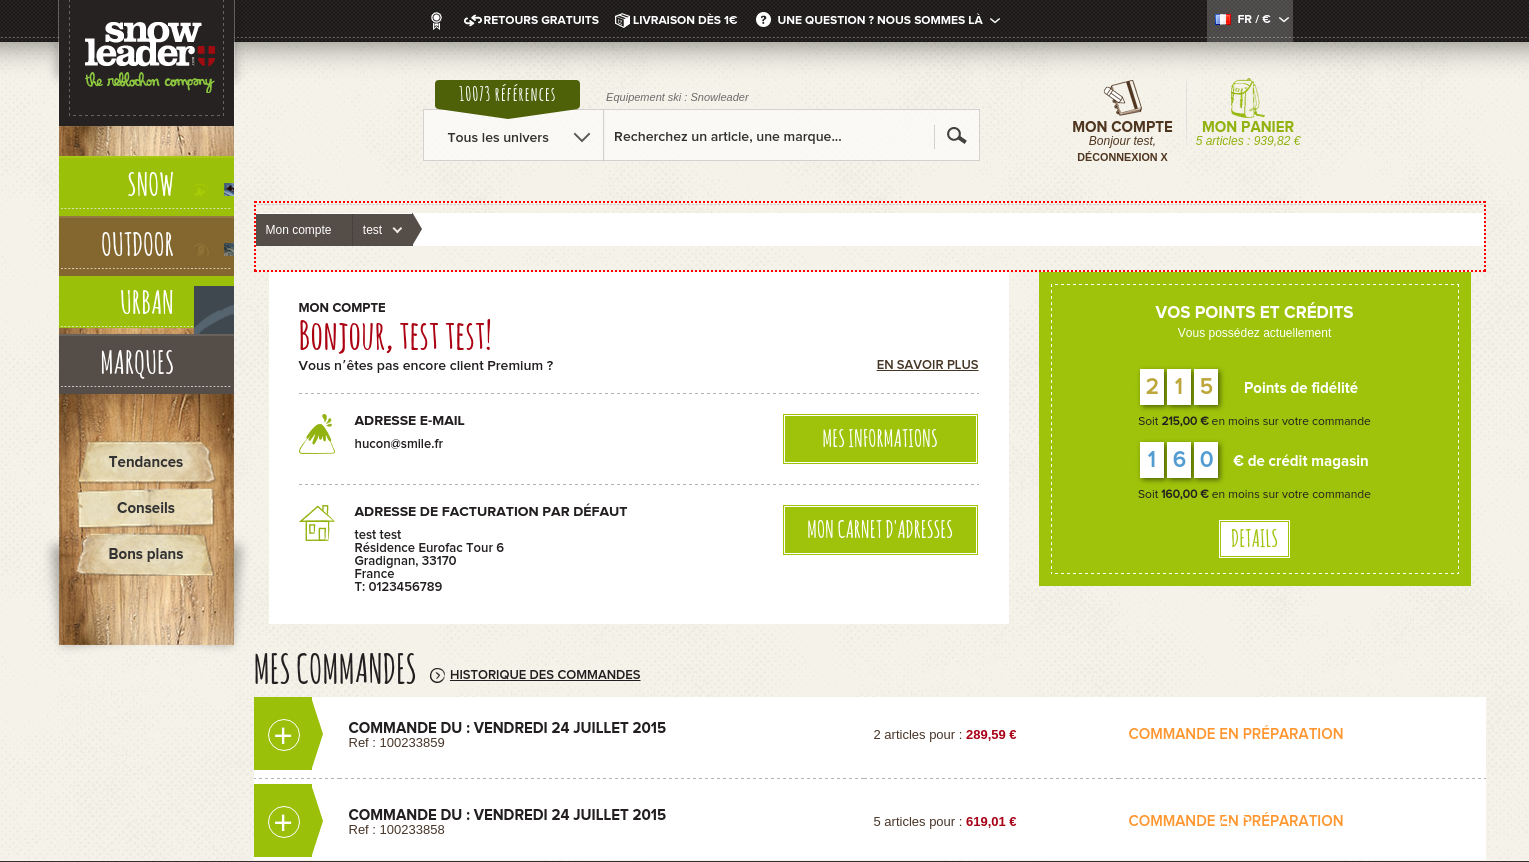
\includegraphics[width=\textwidth]{images/SL_dashboard_customer.png} 
      \captionof{figure}{Dashboard client Snowleader}
      \label{SL_dashboard_customer}
  \end{center}
  
  \newpage
  
  \section*{Annexe Condition sur le lien d'impression de facture}
  \addcontentsline{toc}{section}{Annexe Condition sur le lien d'impression de facture}%Ajout de l'élément dans le sommaire
  \label{SL_print_condition}
  \lstinputlisting[language=html, firstline=1, lastline=7]{SL_print_condition.html}
  \captionof{figure}{Condition sur le lien d'impression de facture}
  
  \newpage
  
  \section*{Annexe Illustration back-office client Magento}
  \addcontentsline{toc}{section}{Annexe Illustration back-office client Magento}%Ajout de l'élément dans le sommaire
  \begin{center}
      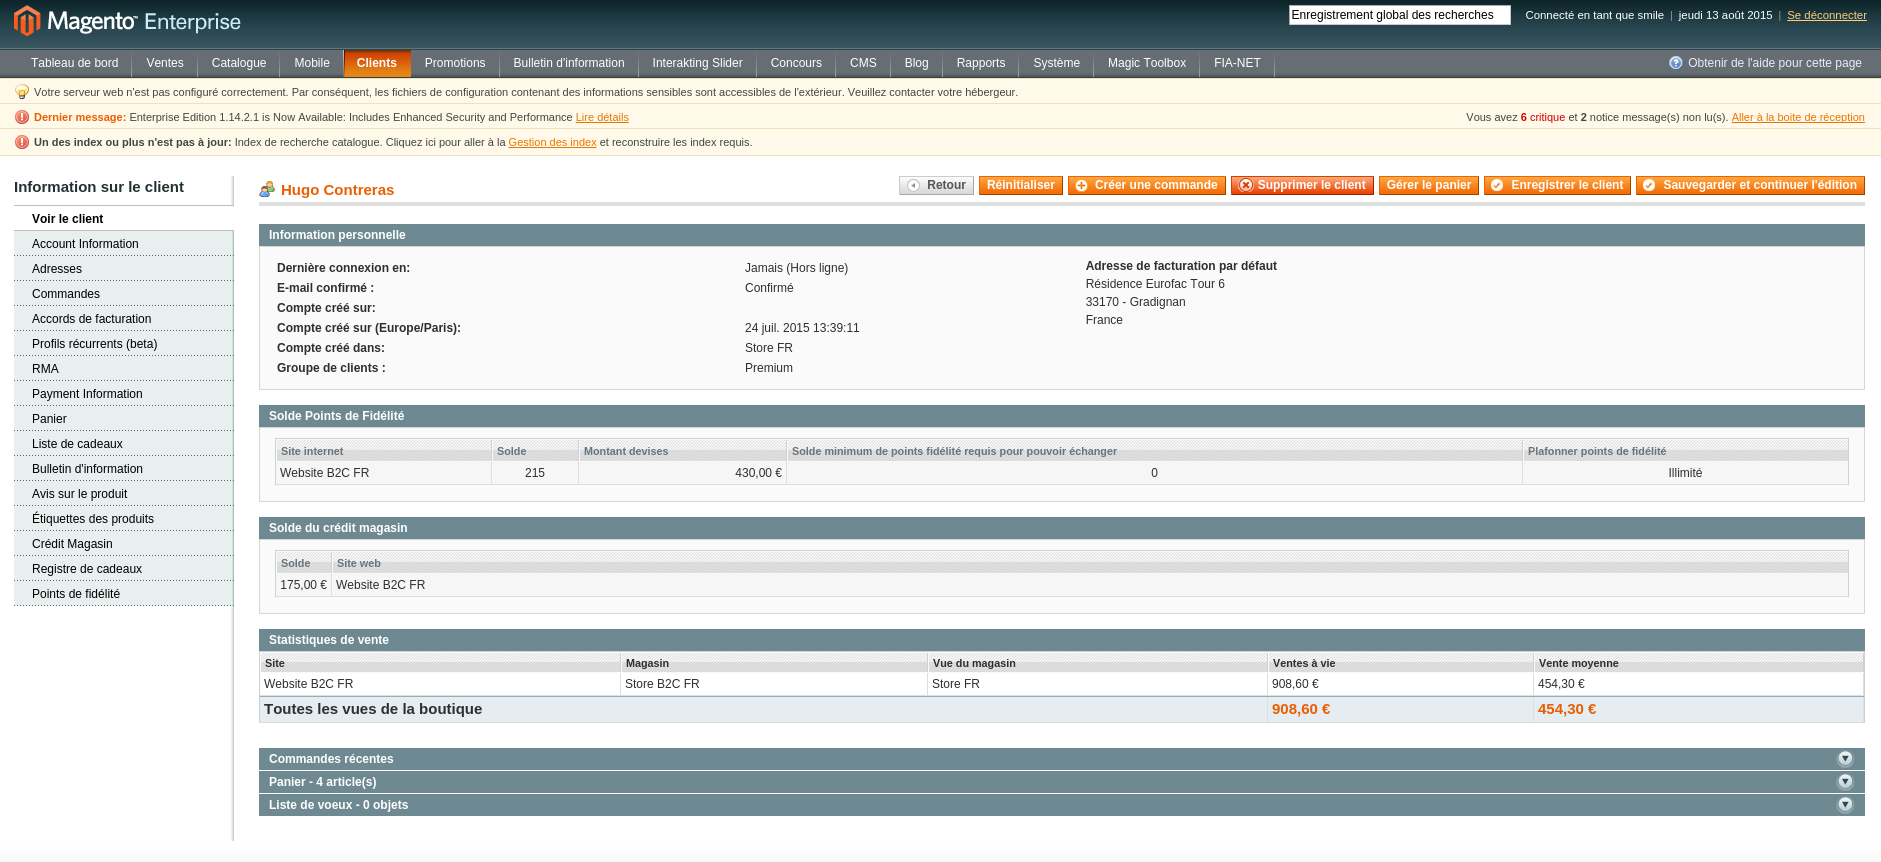
\includegraphics[width=\textwidth]{images/SL_BO_customer.png} 
      \captionof{figure}{Back-office client Magento}
      \label{SL_BO_customer}
  \end{center}
  
  \newpage
  
  \section*{Annexe Déclaration du controller custom loyalty}
  \addcontentsline{toc}{section}{Annexe Déclaration du controller custom loyalty}%Ajout de l'élément dans le sommaire
  \label{SL_loyalty_controller}
  \lstinputlisting[language=php, firstline=1, lastline=174]{SL_loyalty_controller.php}
  \captionof{figure}{Déclaration du controller custom loyalty}
  
  \newpage
  
  \section*{Annexe Illustration formulaire de modification des informations personnelles}
  \addcontentsline{toc}{section}{Annexe Illustration formulaire de modification des informations personnelles}%Ajout de l'élément dans le sommaire
  \begin{center}
      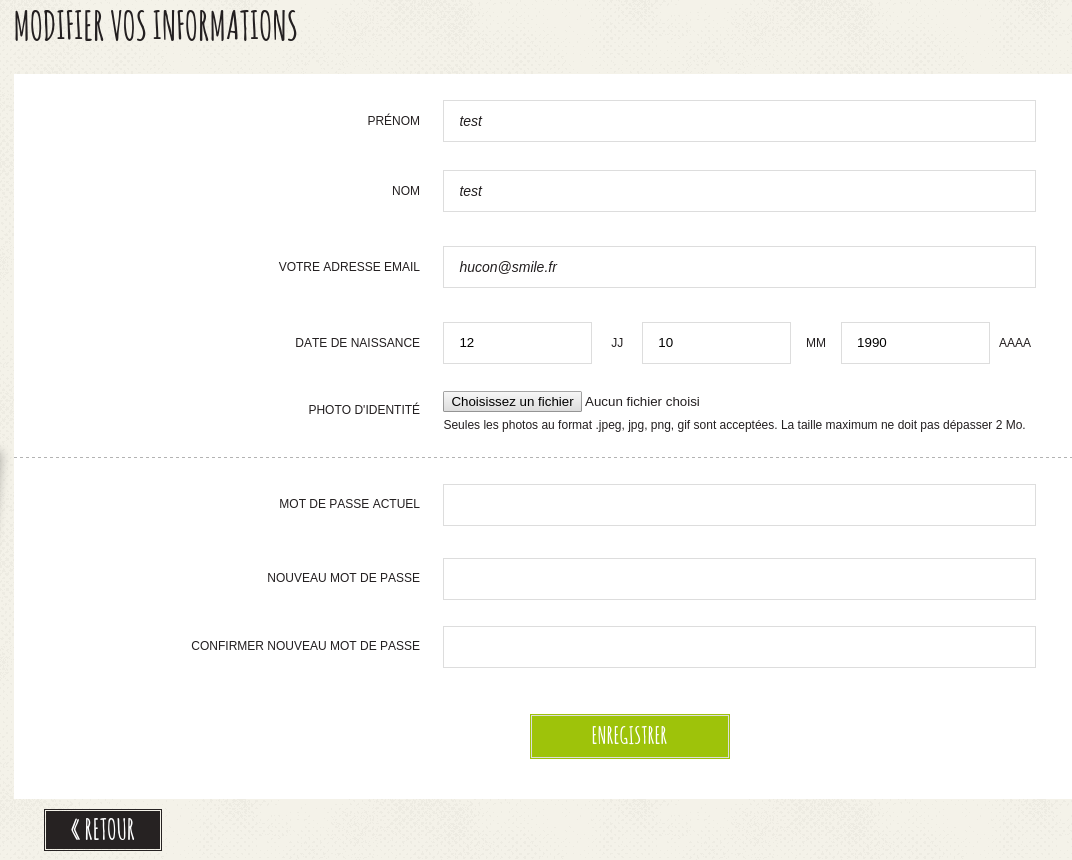
\includegraphics[width=\textwidth]{images/SL_account_information_form.png} 
      \captionof{figure}{Formulaire de modification des informations personnelles}
      \label{SL_account_information_form}
  \end{center}
  
  \newpage
  
  \section*{Annexe Architecture logicielle MVC (Modèle Vue Contrôleur}
  \addcontentsline{toc}{section}{Annexe Architecture logicielle MVC (Modèle Vue Contrôleur}%Ajout de l'élément dans le sommaire
  Le patron d'architecture logicielle modèle-vue-contrôleur, est un modèle destiné à répondre aux besoins des applications interactives en séparant les problématiques liées aux différents composants au sein de leur architecture respective.

  \paragraph*{Modèle}
  Le modèle représente le cœur (algorithmique) de l'application : traitements des données, interactions avec la base de données, etc. Il décrit les données manipulées par l'application. Il regroupe la gestion de ces données et est responsable de leur intégrité. La base de données sera l'un de ses composants. Le modèle comporte des méthodes standards pour mettre à jour ces données (insertion, suppression, changement de valeur). Il offre aussi des méthodes pour récupérer ces données. Les résultats renvoyés par le modèle ne s'occupent pas de la présentation. Le modèle ne contient aucun lien direct vers le contrôleur ou la vue. Sa communication avec la vue s'effectue au travers du patron Observateur.

  Le modèle peut autoriser plusieurs vues partielles des données. Si par exemple le programme manipule une base de données pour les emplois du temps, le modèle peut avoir des méthodes pour avoir tous les cours d'une salle, tous les cours d'une personne ou tous les cours d'un groupe de TD.

  \paragraph*{Vue}
  Ce avec quoi l'utilisateur interagit se nomme précisément la vue. Sa première tâche est de présenter les résultats renvoyés par le modèle. Sa seconde tâche est de recevoir toute action de l'utilisateur (hover, clic de souris, sélection d'un bouton radio, cochage d'une case, entrée de texte, de mouvements, de voix, etc.). Ces différents événements sont envoyés au contrôleur. La vue n'effectue pas de traitement, elle se contente d'afficher les résultats des traitements effectués par le modèle et d'interagir avec l'utilisateur.

  Plusieurs vues peuvent afficher des informations partielles ou non d'un même modèle. Par exemple si une application de conversion de base a un entier comme unique donnée, ce même entier peut être affiché de multiples façons (en texte dans différentes bases, bit par bit avec des boutons à cocher, avec des curseurs). La vue peut aussi offrir à l'utilisateur la possibilité de changer de vue.

  \paragraph*{Contrôleur}
  Le contrôleur prend en charge la gestion des événements de synchronisation pour mettre à jour la vue ou le modèle et les synchroniser. Il reçoit tous les événements de la vue et enclenche les actions à effectuer. Si une action nécessite un changement des données, le contrôleur demande la modification des données au modèle afin que les données affichées se mettent à jour. D'après le patron de conception observateur/observable, la vue est un « observateur » du modèle qui est lui « observable ». Certains événements de l'utilisateur ne concernent pas les données mais la vue. Dans ce cas, le contrôleur demande à la vue de se modifier. Le contrôleur n'effectue aucun traitement, ne modifie aucune donnée. Il analyse la requête du client et se contente d'appeler le modèle adéquat et de renvoyer la vue correspondant à la demande.

  Par exemple, dans le cas d'une base de données gérant les emplois du temps des professeurs d'une école, une action de l'utilisateur peut être l'entrée (saisie) d'un nouveau cours. Le contrôleur ajoute ce cours au modèle et demande sa prise en compte par la vue. Une action de l'utilisateur peut aussi être de sélectionner une nouvelle personne pour visualiser tous ses cours. Ceci ne modifie pas la base des cours mais nécessite simplement que la vue s'adapte et offre à l'utilisateur une vision des cours de cette personne.
  
  \begin{flushright}
    \footnotesize\textit{Source Wikipedia}
  \end{flushright}
  
%Table des illustrations
\listoffigures
\thispagestyle{\chead{}}
\addcontentsline{toc}{chapter}{Table des illustrations}%Ajout de l'élément dans le sommaire

\end{document}